\documentclass[a4paper]{article}

\usepackage{lmodern}

%% Language and font encodings
\usepackage[french]{babel}
\usepackage[utf8x]{inputenc}
\usepackage[T1]{fontenc}
\usepackage{enumitem}
\usepackage{xcolor}
\usepackage{pifont}

%% Sets page size and margins
\usepackage[a4paper,top=3cm,bottom=3cm,left=2cm,right=2cm,marginparwidth=2cm]{geometry}
%% Useful packages
\usepackage{amsmath}
\usepackage{graphicx}
\usepackage[colorinlistoftodos]{todonotes}
\usepackage[colorlinks=true, allcolors=black]{hyperref}
\usepackage{fourier-orns}
\usepackage{titlesec}
\usepackage{fancyhdr}
\usepackage{fancyvrb}
%\renewcommand{\thefootnote}{\*}
\pagestyle{fancy} 
\setcounter{tocdepth}{5}
\usepackage{array}



%% Tikz stuff
\usepackage{tikz}
\usetikzlibrary{calc, arrows}
\tikzstyle{incolore} = [rectangle, rounded corners, draw=black, minimum height=1cm, minimum width=3cm, text width=3cm, text centered]
\usepackage{float}

\usepackage{makecell}
\usepackage{libertine}
\newcommand{\hsp}{\hspace{20pt}}
\newcommand{\HRule}{\rule{\linewidth}{0.5mm}}





\renewcommand{\headrulewidth}{1pt}
\fancyhead[C]{} 
\fancyhead[L]{}
\fancyhead[R]{\footnotesize{\leftmark}}

\renewcommand{\footrulewidth}{1pt}
\fancyfoot[C]{} 
\fancyhead[L]{}
\fancyfoot[R]{\thepage}

\definecolor{Zgris}{rgb}{0.87,0.85,0.85}

\usepackage{eso-pic,graphicx}
\usepackage{xcolor}
\newcommand{\bgimg}[1]{
\AddToShipoutPicture
   {
      \put(\LenToUnit{0 cm},\LenToUnit{0 cm})
      {
            \includegraphics[width=\paperwidth,height=\paperheight]{#1} 
      }
   }
}


\begin{document}


%%\bgimg{Image_15.jpg}





  \begin{titlepage}
    \begin{sffamily}
    \begin{center}
      \textnormal{}\\[6.5cm]
      % Upper part of the page. The '~' is needed because \\
      % only works if a paragraph has started.
      % Title
      \HRule \\[0.4cm]
      { \Huge \bfseries Synthèse\\ Système d'exploitation \\Open Source Th.\\ [0.4cm] }
      \HRule \\[3cm]
      \Large
      Deuxième Bloc\\
      Sécurité des systèmes\\
      Année académique 2020-2021\\[0.2cm]
      \emph{Rédigé par Sénéchal Julien}
      \vfill
      % Bottom of the page
      {\large Fin de rédaction le 18 Décembre 2020}
    \end{center}
    \end{sffamily}
  \end{titlepage}

  \textbf{A savoir avant de commencer à lire la synthèse :}\\
  Vous trouverez beaucoup d'infos que vous jugerez inutiles étant donné que si vous avez suivi les 3 premiers quadrimestres, une bonne partie de la matière est assimilée.
  \\Néanmoins, j'ai préféré reprendre toutes les informations les plus pertinentes et les résumer. (Tables des matières en fin)\\
  A vous de supprimer ce qui ne vous paraît pas utile (genre à l'ancienne vous prenez un fluo quoi xD).
  Alors c'est vrai que la synthèse ressemble plus a un gros résumé qu'à une synthèse mais si ça ne vous plaît pas, vous pouvez toujours la faire vous même xD.\\
  Bonne lecture et bon courage
  \section{A savoir sur Linux}
  \subsection{Qu'est-ce que c'est ?}
  \begin{itemize}[label=\textbullet, font=\Large]
    \item Officiellement le nom de cet OS est \emph{GNU-Linux}, le nom du kernel est \emph{Linux}.
    \item C'est un système multi-tâches \& multi-utilisateur préemptif.
    \item Le kernel \emph{Linux} fut créé sur un noyau de type \emph{UNIX} et basé sur Minix.
  \end{itemize}

  \subsection{Les distributions}
  \subsubsection{Qu'est-ce que c'est ?}
  Une distribution Linux n'est pas une version différente du système Linux, il s'agit juste d'un regroupement d'applications et une présentation
  différente par rapport aux autres distributions (Ex : Kali Linux, Ubuntu, Debian).\\
  
  Difference entre les distributions :
  \begin{itemize}[label=\textbullet, font=\Large]
    \item Liste d'applications pré-installées différente
    \item Méthode de distribution (gratuit, payant, CD-ROM, DVD-ROM, etc...)
    \item Chaque distributions fourni des outils pour son intallation
    \item Ajout de ses propres utilitaires pour faciliter la vie de l'utilisateur
  \end{itemize}

  Une applications qui peut s'éxécuter sur une distribution peut donc s'éxécuter sur chaque distribution Linux. 
  Si elle ne s'éxécute pas, c'est simplement qu'il manque une libraire.

  \subsubsection{Quelques exemples}
  \textbf{Red-Hat}
  \begin{itemize}[label=\textbullet, font=\Large]
    \item La plus connue et une des plus distribuées
    \item A l'origine du système de distribution de packages \emph{RMP}
    \item Evolue vite
    \item Mise à jour et maintenance difficiles (En cause : RPM)\\[0.2cm]
  \end{itemize}
  
  \textbf{Mandrake}
  \begin{itemize}[label=\textbullet, font=\Large]
    \item Basée sur Red-Hat
    \item Orientée utilisateur graphique (optimisée pentium)
    \item Origine française
    \item Facile à installer et "user-friendly"\\[0.2cm]
  \end{itemize}

  \textbf{SuSE}
  \begin{itemize}[label=\textbullet, font=\Large]
    \item Utilise aussi RPM
    \item Connue pour son utilitaire de configuration et d'administration du système \emph{Yast} (système propriétaire)
    \begin{itemize}[label=\ding{228}, font=\scriptsize]
      \item Permet de faire de nombreuses actions qui ne sont pas possible autrement qu'en ligne de commande
    \end{itemize}
    \item Distribuable qu'en CD.\\[0.2cm]
  \end{itemize}

  \textbf{Debian}
  \begin{itemize}[label=\textbullet, font=\Large]
    \item Maintenue par des bénévoles
    \item Une des distribution les plus stable et facile à maintenir (Ouais je sais, j'arrive pas à y croire moi même)
    \begin{itemize}[label=\ding{228}, font=\scriptsize]
      \item Grâce à son système de packages \emph{APT}
    \end{itemize}
    \item Plus complexe et destiné aux utilisateurs plus avancés\\[0.2cm]
  \end{itemize}

  \section{Principes de base}
  \subsection{Comptes utilisateurs}
  \begin{itemize}[label=\textbullet, font=\Large]
    \item Système multi-utilisateurs $\rightarrow$ Plusieurs users peuvent travailler simultanément sur la même machine\\ (grâce à une connexion à distance)
    \item Un compte utilisateur est un ensemble de droits de l'utilisateur et il possède en général son répertoire personnel
    \item Un utilisateur peut faire partie de plusieurs groupes
    \begin{itemize}[label=\ding{228}, font=\scriptsize]
      \item Un groupe permet de définir des droits et des profils pour un ensemble d'utilisateurs
      \item Par défaut, chaque utilisateur appartient à un groupe à son propre nom
    \end{itemize}
    \item Chaque fichier appartient à un utilisateur et un groupe.
    \item 3 niveaux d'accès pour chaque fichier attribuable au propriétaire, au groupe du propriétaire, et aux autres (groupes/users)
    \begin{itemize}[label=\ding{228}, font=\scriptsize]
      \item lecture
      \item écriture
      \item exécution
    \end{itemize}
    \item root $\rightarrow$ super-utilisateur
    \begin{itemize}[label=\ding{228}, font=\scriptsize]
      \item Seul a pouvoir administrer
      \item Accès illimité aux fichiers, ressources, périphériques
    \end{itemize}
  \end{itemize}

    \subsection{Login}
    Une fois l'utilisateur authentifié, il arrive sur le shell qui exécute le fichier de configuration personnel\\ (par exemple : \emph{.bash\_profile} \& \emph{.bashrc})

    \subsection{Arrêt/Démarrage}
    En général, seul \emph{root} peut arrêter le système grâce à 
    \begin{itemize}[label=\textbullet, font=\Large]
      \item shutdown <options> [{<minutes>|now}]
      \item halt 
      \begin{itemize}[label=\ding{228}, font=\scriptsize]
        \item Correspond à passer l'option -h à shutdown et donc arrêter le système
      \end{itemize}
      \item poweroff
      \begin{itemize}[label=\ding{228}, font=\scriptsize]
        \item Correspond à passer l'option -h à shutdown et donc arrêter le système
      \end{itemize}
      \item reboot
      \begin{itemize}[label=\ding{228}, font=\scriptsize]
        \item Correspond à passer l'option -r à shutdown et donc redémarrer le système
      \end{itemize}
    \end{itemize}

    \subsection{Shell}
    C’est la “coquille” qui entoure l’OS et lui permet de communiquer avec l’utilisateur.

    \subsection{Commandes}
    \begin{itemize}[label=\textbullet, font=\Large]
      \item Emploi de commandes très répandu sur un système de type UNIX.
      \item Plus rapide que de naviguer à travers des fenêtres, onglets, etc...
      \item Permet une automatisation avancée (scripts)
    \end{itemize}

    \subsection{All -> Fichier}
    \textbf{TOUT} est considéré comme étant un fichier sous Unix.\\
    Reste la façon de l'utiliser.

    \section{Interface graphique}
    \subsection{Introduction à X}
    \begin{itemize}[label=\textbullet, font=\Large]
      \item La couche graphique n'est qu'une suite d'applications sous Linux
      \item Sous UNIX, l'interface graphique est appelée \emph{X Window}.
      \begin{itemize}[label=\ding{228}, font=\scriptsize]
        \item Fonctions de bases comme le déplacement de la souris, réaction clic souris, affichage, etc...
        \item Ne gère pas les boutons, menus, etc.. qui sont délégués au \emph{Window Manager} (autre application)
      \end{itemize}
    \end{itemize}

    \subsection{Serveur X}
    \begin{itemize}[label=\textbullet, font=\Large]
      \item Fonctionne selon une architecture client-serveur
      \begin{itemize}[label=\ding{228}, font=\scriptsize]
        \item Le client X est l'application qui va demander d'effectuer diverses opération d'affichage
        \item Le serveur X renvoie les informations clavier et souris de l'utilisateur et répond a la demande des clients.
      \end{itemize}
    \end{itemize}

    \subsection{Les gestionnaires de fenêtres}
    \begin{itemize}[label=\textbullet, font=\Large]
      \item Gère les fenêtres affichées à l'écran par le serveur X
      \begin{itemize}[label=\ding{228}, font=\scriptsize]
        \item Placement
        \item Redimensionnement
        \item Fermeture
        \item Décorations des fenêtres
        \item etc...
      \end{itemize}
      \item C'est un client X qui joue le rôle d'intermédiaire entre d'autres client et le serveur X
      \item Exemples : AfterStep, Beryl Fusion, FluxBox, WindowMaker, etc...
    \end{itemize}

    \subsection{Gestionnaires de bureau}
    \begin{itemize}[label=\textbullet, font=\Large]
      \item Les plus célèbres :
      \begin{itemize}[label=\ding{228}, font=\scriptsize]
        \item GNOME
        \item KDE
      \end{itemize}
      \item Couche logicielle permettant d'avoir un bureau (menus avec la liste des programmes, etc...)
    \end{itemize}

    \section{Installation}
    \textbf{Il est conseillé de prendre notes de chaque étapes lors de sa réalisation pour se simplifier la vie en cas de crash ou autre problème dans l'avenir.}
    \subsection{Mise en place du/des FS}
    Il faut au minimum une partition sur le disque pour installer 
    Linux mais il est conseillé d'en avoir au moins une $2^{eme}$ 
    pour le \emph{swap}. \emph{fdisk, cfdisk, Diskdruid, etc...} sont des utilitaires permettant de gérer les partitions.

    \subsection{Partitions}
    La définition des partitions se trouve au niveau du secteur maître d'amorçage (Master Boot Record = MBR). 
    \begin{itemize}[label=\textbullet, font=\Large]
      \item Celui-ci est utilisé pour démarrer le système (contient une partie du code exécuté pour démarrer la machine)
      \item On y trouve aussi \emph{la table des partitions} qui contient toutes les informations de celles-ci (localisatio, taille, etc...)
      \item Le \emph{MBR} occupe les 512 premiers \emph{Bytes} du disque
      \item L'autre partie du MBR est occupée éventuellement par un boot manager (grub, lilo,...) qui gère le démarrage système
      \item Si une partition est marquée comme \emph{active}, le système demarre directement sur celle-ci qui doit alors contenir son propre gestionnaire de démarrage.\\[0.2cm]
    \end{itemize}
    Il existe 3 types de partitions :
    \begin{itemize}[label=\textbullet, font=\Large]
      \item primaire
      \item étendue
      \begin{itemize}[label=\ding{228}, font=\scriptsize]
        \item "Conteneur" a partition logique
      \end{itemize}
      \item logique
    \end{itemize}

    En général on utilise un ou plusieurs partitions primaire. Mais si on désire avoir plus de 4 partitions, on peut définir la dernière partition comme étant une partition
    étendue afin de pouvoir contenir plusieurs partitions logique.\\
    Les partitions primaires sont définies par le \emph{MBR} et les partitions logiques sont chaînées (par manque de place).
    \subsection{Disques \& partitions sous Linux}
    \begin{itemize}[label=\textbullet, font=\Large]
      \item Noms des disques et partitions sous forme de caractères alphanumérique (contrairement a Windows)
      \begin{itemize}[label=\ding{228}, font=\scriptsize]
        \item Disques IDE commencent par "hd"
        \begin{enumerate}
          \item hda 
          \item hdb
          \item ...
        \end{enumerate}
        \item Disques SCSI \& Data commencent par "sd"
        \begin{enumerate}
          \item sda
          \item sdb
          \item ...
        \end{enumerate}
        \item Les disques ou lecteurs branchés sur un port parrallèle (ZIP) ou sur un port USB ou FireWire apparaissent généralement comme des disque SCSI.
      \end{itemize}
      \item Le nom des partitions se composent du noms du disque suivi du numéro de la partition.
      \begin{itemize}[label=\ding{228}, font=\scriptsize]
        \item De 1 à 4 pour les partitions primaires
        \item A partir de 5 pour les partitions logiques
        \item Exemple avec le premier disque SCSI contenant une parition étendue :
      \begin{enumerate}
        \item sda1 - Primaire
        \item sda2 - Primaire
        \item sda3 - Etendue
        \item sda5 - Logique
        \item ...
      \end{enumerate}
    \end{itemize}
    \end{itemize}

    \section{Arborescence \& File System}
    \subsection{Introduction}
    \begin{itemize}[label=\textbullet, font=\Large]
      \item Linux ne distingue pas les disques les uns des autres.
      \begin{itemize}[label=\ding{228}, font=\scriptsize]
        \item Tout le FS possède une racine unique "/", même si il est réparti sur plusieurs disques
        \item Pas de "C:", "D:", "E:" comme sur Windows
      \end{itemize}
      \item Le FS par défaut de Linux est le \emph{ext3} mais de plus en plus le \emph{ext4}
    \end{itemize}
    \subsection{Règles des FS UNIX}
    \begin{itemize}[label=\textbullet, font=\Large]
      \item Chemin d'accès séparés par des "/"
      \begin{itemize}[label=\ding{228}, font=\scriptsize]
        \item Contrairement aux "$\backslash$" sur Windows
      \end{itemize}
      \item Nom de fichier et de repertoire sensible a la casse
      \item Le seul caractère interdit sous Linux est le "/"
      \item Tous les fichiers commençant par un "." sont cachés par défaut (Ex : .bashrc)
      \item Les extensions (.exe, .txt, etc...) jouent un rôle moindre que sur Windows
      \item Les fichiers executable ne sont pas reconnu par leur noms
      \begin{itemize}[label=\ding{228}, font=\scriptsize]
        \item L'execution est un droit du fichier
      \end{itemize}
    \end{itemize}

    \subsection{Arborescence}
    \begin{itemize}[label=\textbullet, font=\Large]
      \item Seul root peut modifier l'Arborescence
      \begin{itemize}[label=\ding{228}, font=\scriptsize]
        \item Sauf les utilisateurs dans leur répertoire personnel
      \end{itemize}
      \item \emph{/bin}
      \begin{itemize}[label=\ding{228}, font=\scriptsize]
        \item Contient les executables binaires servant à l'initialisation du système ainsi que de quelques commandes essentielles.
      \end{itemize}
      \item \emph{/boot}
      \begin{itemize}[label=\ding{228}, font=\scriptsize]
        \item Noyau du système (vmlinuz), les fichiers nécessaires à ce noyau (Ramdisk initrd, etc), et une partie du Boot Loader.
        \item Conseillé de placer ce dossier sur une partition dédié en début de disque
      \end{itemize}
      \item \emph{/dev}
      \begin{itemize}[label=\ding{228}, font=\scriptsize]
        \item Répertoire de fichier spéciaux qui servent de canal de communication avec les périphériques
      \end{itemize}
      \item \emph{/etc}
      \begin{itemize}[label=\ding{228}, font=\scriptsize]
        \item Contient les fichiers de configuration du système et les principaux scripts de démarrage
      \end{itemize}
      \item \emph{/home}
      \begin{itemize}[label=\ding{228}, font=\scriptsize]
        \item Contient tous les répertoires personnels des utilisateurs
      \end{itemize}
      \item \emph{/lib}
      \begin{itemize}[label=\ding{228}, font=\scriptsize]
        \item Contient les bibliothèques et les modules du noyau Linux
      \end{itemize}
      \item \emph{/mnt}
      \begin{itemize}[label=\ding{228}, font=\scriptsize]
        \item racine des points de montage des fichiers périphériques et extérieurs
      \end{itemize}
      \item \emph{/opt}
      \begin{itemize}[label=\ding{228}, font=\scriptsize]
        \item Répertoire d'installation d'application supplémentaire (StarOffice, Java, etc.)
      \end{itemize}
      \item \emph{/proc}
      \begin{itemize}[label=\ding{228}, font=\scriptsize]
        \item pseudo-répertoire créé au boot de la machine qui contient une image du système et permet de dialoguer avec le noyau
      \end{itemize}
      \item \emph{/root}
      \begin{itemize}[label=\ding{228}, font=\scriptsize]
        \item Repertoire personnel du root
      \end{itemize}
      \item \emph{/sbin}
      \begin{itemize}[label=\ding{228}, font=\scriptsize]
        \item Contient les fichiers executables utiles pour l'administration du système
      \end{itemize}
      \item \emph{/tmp}
      \begin{itemize}[label=\ding{228}, font=\scriptsize]
        \item lieu de stockage des fichiers temporaires
      \end{itemize}
      \item \emph{/usr}
      \begin{itemize}[label=\ding{228}, font=\scriptsize]
        \item Programmes accessibles à tous les utilisateurs
        \item Structure reproduisant celle de la racine
      \end{itemize}
      \item \emph{/var}
      \begin{itemize}[label=\ding{228}, font=\scriptsize]
        \item données \textbf{var}iable liées à la machine (logs, spool, etc.)
      \end{itemize}
    \end{itemize}
    \subsection{Référence relative \& Absolue}
    \begin{itemize}[label=\textbullet, font=\Large]
      \item Référence relative
      \begin{itemize}[label=\ding{228}, font=\scriptsize]
        \item Donne le chemin à partir du répertoire de travail courant
        \item Exemple : \textsc{usr@debian$:$/home\$ \space cd user} $\rightarrow$ \textsc{usr@debian$:$/home/user\$}
      \end{itemize}
      \item Référence Absolue
      \begin{itemize}[label=\ding{228}, font=\scriptsize]
        \item Commence par un "/"
        \item Donne le chemin d'accès complet
        \item Exemple : \textsc{usr@debian$:$/home\$ \space cd /etc/network} $\rightarrow$ \textsc{usr@debian$:$/etc/network\$}
      \end{itemize}
    \end{itemize}
    \subsection{Manipuler des fichiers}
    \begin{itemize}[label=\textbullet, font=\Large]
      \item \textsc{touch}
      \begin{itemize}[label=\ding{228}, font=\scriptsize]
        \item Modifier l'heure de dernier accès et dernière modification (si le fichier n'existe pas, il le crée)
      \end{itemize}
      \item \textsc{cp}
      \begin{itemize}[label=\ding{228}, font=\scriptsize]
        \item utilisé pour copier un ou plusieurs fichiers ou répertoires
        \item -p permet de copier les droits d'accès ainsi que le user et groupe propriétaire
        \item -r permet d'appliquer a tout le répertoire et ses sous-répertoire
        \item -i permet d'éviter d'écraser un fichier ayant le même nom que la destination
        \item -u permet d'écraser que si le fichier écrasé est plus ancien
      \end{itemize}
      \item \textsc{mv}
      \begin{itemize}[label=\ding{228}, font=\scriptsize]
        \item permet de déplacer un/des fichier.s/répertoire.s
        \item -u permet de déplacer que les fichiers les plus récents que les fichiers existants à la destination
        \item -i demande confirmation avant d'écraser
      \end{itemize}
      \item \textsc{rm}
      \begin{itemize}[label=\ding{228}, font=\scriptsize]
        \item permet d'effacer des fichiers
        \item -r va permettre d'effacer récursivement un répertoire (tout supprimer dans un dossier ou fichier)
        \item -f va supprimer sans confirmer
        \item -rf efface le contenu d'un répertoire sans confirmation
        \item -i demande confirmation
      \end{itemize}
    \end{itemize}
    \subsection{Afficher le contenu d'un fichier}
    \begin{itemize}[label=\textbullet, font=\Large]
      \item \textsc{cat}
      \begin{itemize}[label=\ding{228}, font=\scriptsize]
        \item affiche le dossier sur la sortie standart
        \item possibilité d'afficher plusieurs fichiers
      \end{itemize}
      \item \textsc{head}
      \begin{itemize}[label=\ding{228}, font=\scriptsize]
        \item affiche les première lignes d'un fichier
        \item -xx pour afficher les xx premières lignes
        \item -v pour imprimer que l'en-tête
        \item possibilité d'afficher les premières lignes de plusieurs fichiers 
      \end{itemize}
      \item \textsc{tail}
      \begin{itemize}[label=\ding{228}, font=\scriptsize]
        \item affiche par défaut les 10 dernières lignes d'un fichier
        \item même option que pour \textsc{head}
      \end{itemize}
      \item \textsc{more}
      \begin{itemize}[label=\ding{228}, font=\scriptsize]
        \item affiche un fichier long écran par écran
        \item \emph{enter} permet d'avancer ligne par ligne
        \item \emph{space} permet d'avancer page par page 
      \end{itemize}
      \item \textsc{less}
      \begin{itemize}[label=\ding{228}, font=\scriptsize]
        \item version GNU de \textsc{more}
        \item beaucoup de fonctionnalités
        \item permet de voyager dans le texte 
        \item permet de faire des recherches en tapant le caractère "/[mot a chercher]"
        \item q pour quitter
      \end{itemize}
      \item \textsc{sort}
      \begin{itemize}[label=\ding{228}, font=\scriptsize]
        \item affiche le contenu par ordre alphabétique
        \item -r = reverse
        \item -u = n'affiche pas les doublons
        \item -b = n'affiche pas les blancs
        \item -f = ignorer les majs
      \end{itemize}
    \end{itemize}
    \subsection{Autres commandes utiles}
    \begin{itemize}[label=\textbullet, font=\large]
      \item \textsc{find}
      \begin{itemize}[label=\ding{228}, font=\scriptsize]
        \item \textsc{find [chemin] expression}
        \item -d affiche les répertoires et pas les fichiers
        \item -f inverse de -d
        \item -name <nom> cherche les fichiers qui portent le nom <nom>. Pour ne pas tenir compte des majs, on utilise -iname <nom>
        \item -size[+/-]<size>
      \end{itemize}
      \item \textsc{locate}
      \begin{itemize}[label=\ding{228}, font=\scriptsize]
        \item fait une recherche grâce a une base de données qui est remise à jour toutes les nuit
        \item plus rapide que find
      \end{itemize}
      \item \textsc{grep}
      \begin{itemize}[label=\ding{228}, font=\scriptsize]
        \item recherche de chaînes de caractères dans des fichiers
        \item -n affiche le numéro de la ligne du résultat
        \item -v affiche les lignes où la chaînes de caractère n'est pas présente
        \item -i ne tient pas compte des maj
        \item -l n'affiche pas les lignes mais le nom du fichier du résultat
        \item -r fait une recherche récursive sur tout le répertoire et les sous-répertoires
      \end{itemize}
      \item \textsc{which}
      \begin{itemize}[label=\ding{228}, font=\scriptsize]
        \item pour trouver le fichier executable d'une commande
      \end{itemize}
      \item \textsc{df}
      \begin{itemize}[label=\ding{228}, font=\scriptsize]
        \item affiche l'espace libre sur le système
        \item -h pour human permet de remplacer la notation en octet par une autre unitée (Go, Mo, etc...)
      \end{itemize}
      \item \textsc{file}
      \begin{itemize}[label=\ding{228}, font=\scriptsize]
        \item affiche le type de données que contient un fichier (image, texte, etc...)
      \end{itemize}
      \item \textsc{split}
      \begin{itemize}[label=\ding{228}, font=\scriptsize]
        \item permet de découper un fichier en plusieurs fichiers séparés
        \item -b permet de choisir la taille max des fichiers générés
      \end{itemize}
      \item \textsc{wc}
      \begin{itemize}[label=\ding{228}, font=\scriptsize]
        \item C'est drôle
        \item permet de compter le nombre de caractères
        \item -c le nombre d'octets
        \item -w de mots
        \item -l de lignes
      \end{itemize}
    \end{itemize}
    \section{Le Shell : BASH}
      \subsection{Shell}
      \subsubsection{Introduction au Shell}
      \begin{itemize}[label=\textbullet, font=\Large]
        \item Interface entre le noyau et l'utilisateur
        \item BASH = Bourne Again Shell, c'est le Shell par défaut sur Linux (lancé par la commande /bin/bash)
        \item Peut être changé selon l'utilisateur
        \begin{itemize}[label=\ding{228}, font=\scriptsize]
          \item Pour savoir le Shell affecté a un user $\rightarrow$ /etc/passwd\\[0.2cm]
        \end{itemize}
    \end{itemize}
    Ordre d'analyse d'une commande :
    \begin{enumerate}
      \item Lors de l'entrée d'une commande, le shell va vérifier si celle-ci est une commande interne (voir \emph{man bash})
      \item Ensuite il vérifie les alias
      \begin{itemize}[label=\ding{228}, font=\scriptsize]
        \item Pour définir un \emph{alias} on utilise la commande \emph{alias} (Cette méthode crée un alias temporaire)
      \end{itemize}
      \item Enfin, il cherche un programme exécutable qui porte le même nom que la commande sur le FS en se servant des chemin d'accès listés dans \textbf{\$PATH}
      (variable d'environnement)
      \item Si il trouve, il execute en lui passant les arguments spécifiés sur la ligne de commande
      \begin{itemize}[label=\ding{228}, font=\scriptsize]
        \item Par sécurité, le répertoire courant est toujours exclu du Path
      \end{itemize}
    \end{enumerate}

    \subsubsection{Lancer des commandes dans le Shell}
    \begin{itemize}[label=\textbullet, font=\Large]
      \item Les commandes sont la plus part du temps des commandes externes, ce sont donc de simples programmes exécutables
      \item Pour lancer une commande, on tape simplement son nom
      \item L'espace entre le nom de la commande et le premier argument est obligatoire
      \item Différents type d'arguments
      \begin{itemize}[label=\ding{228}, font=\scriptsize]
        \item Les Options : modifient le comportement d'une commande\\ Elle sont généralement non obligatoire, et sous Linux elles sont souvent précédées par un "-"
        \item Les aides : -h ou --help
      \end{itemize}
    \end{itemize}

    \subsubsection{L'environnement des commandes}
    L'environnement de la ligne de commande est initialisé par une série de script :
    \begin{itemize}[label=\textbullet, font=\Large]
      \item \textsc{/etc}
      \begin{itemize}[label=\ding{228}, font=\scriptsize]
        \item fichiers dont les noms sont du genre bash, profiles, etc. qui sont des scripts pour tous les utilisateurs
      \end{itemize}
      \item \textsc{/home/[répertoire personnel]}
      \item \begin{itemize}[label=\ding{228}, font=\scriptsize]
        \item fichiers dont les noms sont du genre bash, profiles, etc. qui sont des scripts pour un utilisateur en particulier
      \end{itemize}
    \end{itemize}

    \subsubsection{Les caractères spéciaux}
    \begin{figure}[H]
    \centering
    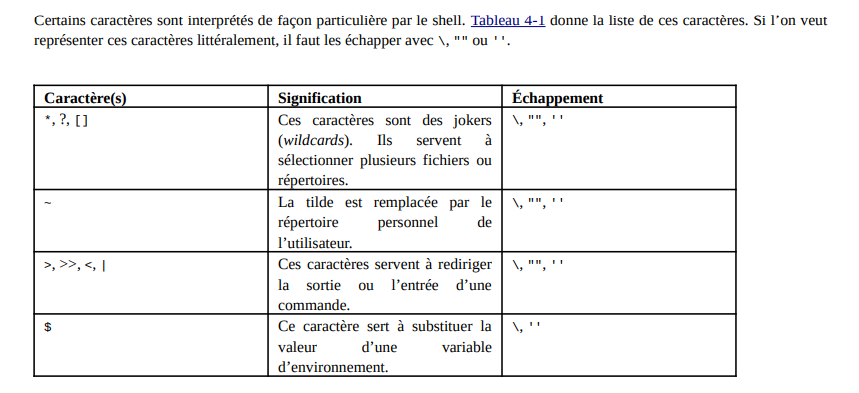
\includegraphics[width=17cm]{images/cours.PNG}
    \caption{caractères spéciaux}
    \end{figure}

    \subsubsection{Les wildcars ou Jokers}
    \begin{itemize}[label=\textbullet, font=\Large]
      \item * $\rightarrow$ n’importe quelle suite d’un nombre quelconque de caractères
      \item ? $\rightarrow$ n'importe quel caractère unique
      \item \textasciitilde \space $\rightarrow$ raccourci pour le répertoire personnel
      \begin{itemize}[label=\ding{228}, font=\scriptsize]
        \item \textsc{ \textasciitilde \space jean} $\rightarrow$ renvoie vers le répertoire personnel de "jean"
      \end{itemize}
      \item $\left\lbrack \space \space \right\rbrack$ $\rightarrow$ un caractère parmi ceux étant entre les crochets
      \begin{itemize}[label=\ding{228}, font=\scriptsize]
        \item $\left\lbrack aY \right\rbrack$ $\rightarrow$ a ou Y
        \item $\left\lbrack a-d \right\rbrack$ $\rightarrow$ un caractère entre a et d (a et d compris)
      \end{itemize}
      \item $\backslash$ $\rightarrow$ permet d'échapper à un caractère spécial
      \begin{itemize}[label=\ding{228}, font=\scriptsize]
        \item Par exemple \textsc{$\backslash$?} permet de prendre le caractère "?" et de le traiter comme un caractère normal
      \end{itemize}
      \item \$ $\rightarrow$ correspond au début d'une variable d'environnement
      \begin{itemize}[label=\ding{228}, font=\scriptsize]
        \item Propre à l'environnement en cours\\[0.2cm]
      \end{itemize}

    \end{itemize}

    Pour plus d'infos sur les jokers : \textsc{man 7 glob}

    \subsubsection{Variables d'environnement}
    \begin{itemize}[label=\textbullet, font=\Large]
      \item Les variables d'environnement peuvent être modifiés et paramétrées par l'utilisateur
      \item Pour afficher les variables d'environnement, commande : \textsc{set}
      \item Pour définir une variable d’environnement : \textsc{export globalvar}
      \item Pour supprimer une variable d’environnement : \textsc{unset globalvar}
    \end{itemize}
    \subsection{Les commandes de BASH}
    \subsubsection{Historique}
    \begin{itemize}[label=\textbullet, font=\Large]
      \item Maintient d'un Historique
      \begin{itemize}[label=\ding{228}, font=\scriptsize]
        \item Pour revenir sur une commande précédemment tapée on utilise les flèche directionnelles
      \end{itemize}
      \item Le point d’exclamation placé en début de commande indique à Bash de
      compléter la ligne en utilisant la dernière commande qui commence par ce qui à été tapé après le "!"
      \item La commande \textsc{history} permet d'affichier l'historique des commandes
    \end{itemize}
    \subsubsection{Complétion des commandes}
    \begin{itemize}[label=\textbullet, font=\Large]
      \item Permet de compléter un mot (commande ou nom de fichier) grâce à \emph{TAB}
      \begin{itemize}[label=\ding{228}, font=\scriptsize]
        \item Sur certaines distributions est fourni un jeux de scripts qui permet une auto complétion avancée. Elle peux par ex. afficher les
        options d''une commande, ou les fichiers reconnus par cette commande (ex : les fichiers zip avec unzip). C’est le cas p.ex. De
        la debian. Il s’agit d’un option non activée par défaut, il faut décommenter certaines lignes pour pourvoir l’employer
      \end{itemize}
    \end{itemize}
    \subsubsection{Touches reconnues par le shell}
    \begin{itemize}[label=\textbullet, font=\Large]
      \item \emph{ENTER}
      \item \emph{BACKSPACE}
      \item \emph{CTRL-U} (efface la ligne)
      \item \emph{CTRL-C}
    \end{itemize}
    \subsection{Toutes les infos sur Linux}
    \subsubsection{L'aide}
    \begin{itemize}[label=\textbullet, font=\Large]
      \item \textsc{--help}
      \item \textsc{-?}
      \item \textsc{-h}
    \end{itemize}
    \subsubsection{man}
    \begin{itemize}[label=\textbullet, font=\Large]
      \item \textsc{man [N}\degres \textsc{ section] <commande>} -> affiche le manuel de la commande
      \item Les man pages sont séparées en sections, numérotées de 1 à 9
      \begin{itemize}[label=\ding{228}, font=\scriptsize]
        \item Section 1 : Documentation sur les commandes accessibles aux utilisateurs normaux
        \item Section 2 à 7 : Informations utiles aux développeurs
        \item Section 8 : Documentation sur les commandes utiles à l'administration système
        \item D’autres sections existent, mais elles ne contiennent généralement pas d’informations utiles à un
        utilisateur moyen.
      \end{itemize}
      \item Stocké dans \textsc{/usr/share/man}
    \end{itemize}

    \subsubsection{info}
    \begin{itemize}[label=\textbullet, font=\Large]
      \item Autre système d'aide en ligne
      \item Toutes les commandes n'ont pas de page info
      \item Utilise un système hypertexte qui facilite la navigation
    \end{itemize}

    \subsubsection{apropos}
    Cette commande permet de voir toute la documentation se rapportant à un terme. Cela permet de s’y
retrouver une commande par exemple
    \subsubsection{La documentation}
    Se trouve dans \textsc{/usr/share/doc}

    \subsection{Entrée \& sortie standart}
    \subsubsection{Redirections}
    \begin{itemize}[label=\textbullet, font=\Large]
      \item >
      \begin{itemize}[label=\ding{228}, font=\scriptsize]
        \item redirige la sortie standard vers un fichier (écrase le contenu du fichier)
        \item sortie standard = écran
      \end{itemize}
      \item >>
      \begin{itemize}[label=\ding{228}, font=\scriptsize]
        \item redirige la sortie en ajoutant les données au fichier (n'écrase donc pas)
      \end{itemize}
      \item <
      \begin{itemize}[label=\ding{228}, font=\scriptsize]
        \item redirige l'entrée standard depuis un fichier
        \item rmdir < RépertoireQuiDoitEtreEffacé
      \end{itemize}
      \item 2> ou 2>>
      \begin{itemize}[label=\ding{228}, font=\scriptsize]
        \item redirige l'erreur standart
        \item erreur standart = moniteur par défaut
      \end{itemize}
      \item > fichier 2> \&1
      \begin{itemize}[label=\ding{228}, font=\scriptsize]
        \item redirige la sortie standard et l'erreur vers un fichier
      \end{itemize}
      \item >> fichier 2> \&1
      \begin{itemize}[label=\ding{228}, font=\scriptsize]
        \item ajoute la sortie standard et l'erreur a la suite du fichier
      \end{itemize}
    \end{itemize}

    \subsubsection{Pipes}
    \begin{itemize}[label=\textbullet, font=\Large]
      \item |
      \begin{itemize}[label=\ding{228}, font=\scriptsize]
        \item redirige la sortie d'une commande vers une autre
      \end{itemize}
    \end{itemize}

    \subsubsection{Tee}
    \begin{itemize}
      \item redirige vers la sortie standard et vers tous les fichiers donné en argument
    \end{itemize}

    \subsubsection{Editeur de texte}
    \emph{VIM} mais pas plus d'info ici :-)

    \section{Gestion des paquets}
    \begin{itemize}[label=\textbullet, font=\Large]
      \item RPM
      \begin{itemize}[label=\ding{228}, font=\scriptsize]
        \item Système de gestion de paquet pour RedHat
        \item Détecte les dépendances sans les gérer
        \item Installe/Désinstalle/Mets à jour a partir d'un fichier "rpm"
      \end{itemize}
      \item yum
      \begin{itemize}[label=\ding{228}, font=\scriptsize]
        \item Surcouche a RPM
        \item Apporte des fonctionnalités similaire à APT
      \end{itemize}
      \item Dpkg
      \begin{itemize}[label=\ding{228}, font=\scriptsize]
        \item Equivalent "RPM" pour Debian
        \item Système de gestion des paquets
        \item Détecte les dépendances sans les gérer
        \item Installe/Désinstalle/Mets à jour a partir d'un fichier "deb"
      \end{itemize}
      \item APT
      \begin{itemize}[label=\ding{228}, font=\scriptsize]
        \item Gestionnaire de paquets de distribution chez Debian
        \item Gère les dépendances
        \item Possibilité de mélanger les versions de distribution (ex: version unstable chez Samba pour avoir l'accès à certaines fonctionnalités)
        \item Possibilité de créer un fichier "preferences" (\textsc{/etc/apt/preferences} ou créer un fichier dans \textsc{/etc/apt/preferences.d})
        \item Syntaxe (à connaître) :\\\textsc{Package : *\\Pin : release a=\emph{[version]}\\Pin-Priority : [Priorité]}
        \begin{itemize}
          \item " * " : Tous les paquets (peut être remplacé par un paquet spécifique)
          \item version : stable/stretch/testing\\ (stable/lors du passage à la nouvelle version de Debian, la version des paquets de stretch sera préférée à la
          nouvelle stable/en test)
          \item Priorité :
        \end{itemize}
      \end{itemize}
    \end{itemize}
    \begin{center}
      

    \begin{tabular}{|l|r|}
      \hline
      \makecell[c]{\textbf{Priorité}} & \makecell[c]{\textbf{Installé si *}}\\
      \hline
      0-100 &  \makecell[l]{aucune version ne l'est déjà}\\
      \hline
      100-500 & \makecell[l]{pas de version plus récente installé ou disponible}\\
      \hline
      500-990 & \makecell[l]{pas de version plus récente installée ou disponible dans la version choisie (stable/testing/etc...)}\\
      \hline
      990-1000 & \makecell[l]{pas de version plus récente installée}\\
      \hline
      > 1000 & \makecell[l]{priorité d'un paquet déjà installé}\\
      \hline
      valeurs égale & \makecell[l]{prend le paquet le plus récent}\\ 
      \hline
    \end{tabular}\\
  \end{center}
    \scriptsize{Pas d'info sur les paquets binaire et paquets sources}
    \normalsize
    \section{Users and groups}
    Plusieurs élément ne seront pas cité dans ce chapitre parce que ces points devraient déjà être connu.
    \subsection{La base}
    \begin{itemize}[label=\textbullet, font=\Large]
      \item \textsc{UID}
      \begin{itemize}[label=\ding{228}, font=\scriptsize]
        \item Identificateur numérique d'un utilisateur (seul manière de reconnaître les utilisateurs pour le kernel)
        \item Possède un nom d'utilisateur (login)
        \item UID 0 = Root
        \item Seul root peut passer outre les droits des fichiers et ce même si les utilisateurs ont des droits étendu
      \end{itemize}
      \item \textsc{GID}
      \begin{itemize}[label=\ding{228}, font=\scriptsize]
        \item Identificateur numérique pour les groupes
        \item Même particularité que les UID
        \item Un utilisateur appartient à un groupe primaire et peut appartenir des groupes secondaires
      \end{itemize}
      \item La commande \textsc{id} permet d'obtenir le UID et les GID de l'utilisateur courant. \textsc{id [nom d'utilisateur]} permet d'avoir les infos de l'utilisateur en question
      \item Création de nombreux comptes et groupes lors de l'installation
      \begin{itemize}[label=\ding{228}, font=\scriptsize]
        \item Permet d'attribuer un utilisateurs à un deamon (parfois ce n'est pas le cas et le processus reçoit un propriétaire, le processus est lancé en SUID ou SGID (genre de su))
        \item Permet de limiter les risques de sécurité étant donné que chaque compte est restreint
      \end{itemize}
    \end{itemize}
    \subsection{Fichiers concernés}
    \begin{itemize}
      \item \textsc{/etc/passwd}
      \begin{itemize}[label=\ding{228}, font=\scriptsize]
        \item Login
        \item MDP
        \item UID
        \item GID
        \item Nom complet + coordonnées
        \item Emplacement du "home"
        \item Shell utilisé (Optionnel)
      \end{itemize}
      \item \textsc{/etc/shadow}
      \begin{itemize}[label=\ding{228}, font=\scriptsize]
        \item login
        \item Hash du mdp + salt (si = à * ou !, alors le compte est désactivé)
        \item n jours depuis le dernier changement de mdp (compté à partir du 1er Janvier 1970 (WTF))
        \item n jours à attendre avant de de pouvoir changer de mdp
        \item n jours avant la fin de validité du mdp (et pendant lesquels il sera averti)
        \item n jours après la fin de validité provoquant la désactivation du compte
        \item n jours depuis que le compte est désactivé (compté à partir du 1er Janvier 1970 (Je piges par pourquoi autant d'exagération))
        \item Champ Réservé
      \end{itemize}
      \item \textsc{/etc/group}
      \begin{itemize}[label=\ding{228}, font=\scriptsize]
        \item Nom du groupe
        \item mdp chiffré éventuel
        \item GID
        \item Liste des logins appartenant au groupe
      \end{itemize}
    \end{itemize}
    \subsection{Changer le mot de passe}
    \begin{itemize}
      \item commande \textsc{passwd}
      \item Bonne stratégie de mdp
      \begin{itemize}[label=\ding{228}, font=\scriptsize]
        \item > 10 caractères
        \item éviter les mot du dictionnaire (même inversé ou avec certains caractères en maj)
        \item éviter les mots de passes évidents
        \item Mélanger les différents types de caractères
        \item Ne pas réutiliser de mot de passe
        \item Le changer régulièrement
      \end{itemize}
    \end{itemize}
    \subsection{Limiter l'usage d'un compte}
    Respectivement les options -l et -u à \textsc{passwd}. Et pour désactiver le shell il faut le modifier par défaut dans le \textsc{/etc/passwd}.
    \subsection{Modifier les propriétés d'un compte}
    \begin{itemize}
      \item \textsc{usermod}
      \item Exemple :
      \begin{itemize}[label=\ding{228}, font=\scriptsize]
        \item usermod -G liste, des, groupes, secondaires
        \item usermod -g groupe\_primaire
      \end{itemize}
    \end{itemize}
    \subsection{Informations sur les utilisateurs}
    \begin{itemize}[label=\textbullet, font=\Large]
      \item who \& users \& w
      \begin{itemize}[label=\ding{228}, font=\scriptsize]
        \item Commandes permettant d'avoir des infos sur les utilisateurs connectés (w donnant plus d'infos)
      \end{itemize}
      \item whoami
      \begin{itemize}[label=\ding{228}, font=\scriptsize]
        \item Commandes permettrant de savoir qui on est
      \end{itemize}
      \item last [-n x]
      \begin{itemize}[label=\ding{228}, font=\scriptsize]
        \item Historique de connexions (ou des x dernières connexions)
      \end{itemize}
      \item lastlog
      \begin{itemize}[label=\ding{228}, font=\scriptsize]
        \item le nom parle de lui même (sans argument liste tous les users)
      \end{itemize}
      \item ac
      \begin{itemize}[label=\ding{228}, font=\scriptsize]
        \item Temps de connexion des utilisateurs
      \end{itemize}
      \item fail \& faillog
      \begin{itemize}[label=\ding{228}, font=\scriptsize]
        \item Comme pour last et lastlog mais pour les tentatives de connexion échouées
      \end{itemize}
    \end{itemize}
    Le système retrouve toutes ces informations grâces aux divers fichiers :
    \begin{itemize}[label=\textbullet, font=\Large]
      \item Pour les connexions réussies
      \begin{itemize}[label=\ding{228}, font=\scriptsize]
        \item \textsc{/var/run/utmp}
        \begin{itemize}
          \item Une entrée est créé lors de chaque connexion et supprimée à la déconnexion
        \end{itemize}
        \item \textsc{/var/log/wtmp}
        \begin{itemize}
          \item Contient toutes les connexions et déconnexions
        \end{itemize}
        \item \textsc{/var/log/lastlog}
        \begin{itemize}
          \item Date de dernière connexion classé par UID
        \end{itemize}
      \end{itemize}
      \item Pour les connexions échouées
      \begin{itemize}[label=\ding{228}, font=\scriptsize]
        \item \textsc{/var/log/btmp}
        \item \textsc{/var/log/faillog}
      \end{itemize}
    \end{itemize}

    \section{Gestion avancées des fichiers}
    \subsection{Droits spéciaux}
    \begin{itemize}[label=\textbullet, font=\Large]
      \item s
      \begin{itemize}[label=\ding{228}, font=\scriptsize]
        \item permet d'exécuter un fichier avec les droits du propriétaire (Set-UID ou SUID / Set-GUID ou SGUID)
      \end{itemize}
      \item t
      \begin{itemize}[label=\ding{228}, font=\scriptsize]
        \item ne sert que sur les répertoires et donne le droit de supprimer le fichier qu'a son propriétaire (sticky-bit)
      \end{itemize}
    \end{itemize}
    Je passe tout ce qui est chmod, chown, et l'umask étant donné que je connais déjà très bien et que flemme.
    \subsection{Inodes}
      Pour vérifier les inodes : ls -i et df -i
    \subsection{Types de fichiers}
    \begin{itemize}[label=\textbullet, font=\Large]
      \item fichier normal
      \begin{itemize}[label=\ding{228}, font=\scriptsize]
        \item texte, executable, etc..
      \end{itemize}
      \item fichier répertoire
      \item fichier lien symbolique
      \begin{itemize}[label=\ding{228}, font=\scriptsize]
        \item fichier qui contient un pointeur vers un autre fichier (comme un raccourci windows)
      \end{itemize}
      \item fichier spécial (de périphériques)
      \begin{itemize}[label=\ding{228}, font=\scriptsize]
        \item fichier qui permet l'accès à un périphériques, une partition (ex: /dev/sdb).
        \item Les fichiers de ce type sont dans /dev
      \end{itemize}
    \end{itemize}

      \subsection{Lien}
      \subsubsection{Liens durs}
      Un lien dur associe un ou plusieurs fichiers à un même espace disque sur un système de fichier. Ils permettent :
      \begin{itemize}[label=\textbullet, font=\Large]
        \item d'avoir un fichier dans un répertoire
        \item d'avoir plusieurs nom pour un programme et de réagir en fonction de son nom d'appel
        \item à un inode de se trouver dans plusieurs répertoires différents
        \item à ne pas avoir un fichier en "double" sur le disque
      \end{itemize}
      \subsubsection{Liens symboliques}
      \begin{itemize}[label=\textbullet, font=\Large]
        \item Chemin symbolique pointant vers un autre fichier ou répertoire
        \item Indépendant du FS
        \item Agis comme une sorte de "raccourci"
      \end{itemize}
      \subsection{Liste des fichiers périphériques}
      \begin{center}
        \begin{tabular}{|l|r|}
          \hline
          \makecell[c]{\textbf{Chemin d'accès}} & \makecell[c]{\textbf{Type de périphérique}}\\
          \hline
          \makecell[c]{/dev/hd/...} & \makecell[l]{Périphériques IDE selon l'odre des bus}\\
          \hline
          \makecell[c]{/dev/cdrom...} & \makecell[l]{Raccourcis vers le lecteur de CD-ROM}\\
          \hline
          \makecell[c]{/dev/sd...} & \makecell[l]{Périphériques SCSI, USB, SATA}\\
          \hline
          \makecell[c]{/dev/scd…} & \makecell[l]{CD-ROM SCSI}\\
          \hline
          \makecell[c]{/dev/ttyS…} & \makecell[l]{Ports séries}\\
          \hline
          \makecell[c]{/dev/tty…} & \makecell[l]{Consoles virtuelles}\\
          \hline
          \makecell[c]{/dev/psaux } & \makecell[l]{Port PS/2}\\
          \hline
          \makecell[c]{/dev/mouse} & \makecell[l]{Lien vers la souris}\\
          \hline
          \makecell[c]{/dev/fd…} & \makecell[l]{Lecteurs disquettes}\\
          \hline
          \makecell[c]{/dev/par..} & \makecell[l]{Ports parallèles}\\
          \hline
          \makecell[c]{/dev/lp…} & \makecell[l]{Imprimantes parallèles}\\
          \hline
          \makecell[c]{/dev/random} & \makecell[l]{Périphérique aléatoire : génére des valeurs pseudo aléatoires}\\
          \hline
          \makecell[c]{/dev/zero} & \makecell[l]{Périphérique qui génére des zéros}\\
          \hline
          \makecell[c]{/dev/null } & \makecell[l]{Périphérique vide. Tout ce qui y rentre disparaît}\\
          \hline
          \makecell[c]{/dev/loop} & \makecell[l]{Périphérique de boucle de montage}\\
          \hline
        \end{tabular}
        
      \end{center}

      \subsection{Numéro de périphériques}
      \begin{itemize}[label=\textbullet, font=\Large]
        \item C'est \textsc{udevd} qui gère les numéros de périphériques.
        \item C'est par ce numéro que le système reconnaît le type du fichier de périphérique et sait comment y accéder.
        \item Le numéro est interprété par le "driver" du périphérique
      \end{itemize}

      \section{Gestion des systèmes de fichiers}
      \subsection{Outils de partitionnement}
      \begin{itemize}[label=\textbullet, font=\Large]
        \item fdisk
        \begin{itemize}[label=\ding{228}, font=\scriptsize]
          \item commande traditionnelle de partitionnement
          \item -l pour lister les partitions
        \end{itemize}
        \item cfdisk
        \begin{itemize}[label=\ding{228}, font=\scriptsize]
          \item plus convivial
        \end{itemize}
        \item sfdisk
        \begin{itemize}[label=\ding{228}, font=\scriptsize]
          \item permet de tout faire (d'après le prof c'est le couteau suisse du partitionnement)
        \end{itemize}
      \end{itemize}
      Le kernel doit être mis au courant des modifications apportées et cela grâce à un reboot ou via les commandes partprobe ou sfdisk.

      \subsection{Systèmes de fichiers}
      \begin{itemize}[label=\textbullet, font=\Large]
        \item mkfs
        \begin{itemize}[label=\ding{228}, font=\scriptsize]
          \item Outil permettant de créer des systèmes de fichiers
          \item Existe des versions différents pour chaque FS (ex : mk2fs ou mkfs.ext2)
          \item -c pour rechercher les blocs défectueux et les marquer comme non utilisables
        \end{itemize}
      \end{itemize}

      \subsection{Montages}
      \begin{itemize}[label=\textbullet, font=\Large]
        \item mount
        \begin{itemize}[label=\ding{228}, font=\scriptsize]
          \item permet d'accéder a un système de fichier (partition, périphériques, etc...) en l'intégrant dans l'arborescence (ex : /dev/sdb)
        \end{itemize}
        \item umount
        \begin{itemize}[label=\ding{228}, font=\scriptsize]
          \item démonte un FS monté
          \item Pour ça il ne doit plus être occupé
          \item La commande "lsof" permet de lister tous les fichiers ouvert
          \item Pour les fichiers ouvets dans le home
          \begin{itemize}
            \item lsfo | grep /home
          \end{itemize}
        \end{itemize}
        \item /etc/fstab
        \begin{itemize}[label=\ding{228}, font=\scriptsize]   
          \item fichier où sont précisé les fichiers à monter au démarrage
        \end{itemize}
        \item /etc/mtab
        \begin{itemize}[label=\ding{228}, font=\scriptsize]   
          \item liste des systèmes de fichiers actuellement montés
        \end{itemize}
      \end{itemize}
      \subsection{Taille des partitions}
      \begin{itemize}[label=\textbullet, font=\Large]
        \item /boot : 100MB
        \item /var : 2GB (permet de séparer les logs et ainsi assurer la stabilité système)
        \item /tmp : 500MB (like /var)
        \item /usr : pas d'info apparremment. Pourquoi faire au fond :/
        \item /home : 90GB selon le nombre d'utilisateur
        \item SWAP :
        \begin{itemize}[label=\ding{228}, font=\scriptsize] 
          \item Si - de 2GB de ram : 2 fois la taille de la ram
          \item Entre 2 et 4 GB de ram : 2G en + de la ram
          \item Entre 6 et 8 GB de ram : taille de la ram
          \item Si + de 8 GB de ram : 1/2 de la ram (si vous avez une explication je prends)
        \end{itemize}
      \end{itemize}

      \subsection{Gestion des quotas}
      \subsubsection{Différentes limites de quota}
      \begin{itemize}[label=\textbullet, font=\Large]
        \item Limite dure par utilisateur (hard limit)
        \begin{itemize}[label=\ding{228}, font=\scriptsize] 
          \item Max qui ne peut jamais être dépassé
        \end{itemize}
        \item Limite douce par utilisateur (soft limit)
        \begin{itemize}[label=\ding{228}, font=\scriptsize] 
          \item Limite a partir de laquelle un utilisateur pourra continuer a écrire sur le disque et recevra des avertissements
        \end{itemize}
        \item Limite dure par groupe
        \begin{itemize}[label=\ding{228}, font=\scriptsize] 
          \item Limite max du groupe, et ce même si un utilisateur n'as pas remplit son quota
        \end{itemize}
        \item Limite douce par groupe
        \begin{itemize}[label=\ding{228}, font=\scriptsize] 
          \item same as soft limit
        \end{itemize}
        \item Temps de grâce (grace period)
        \begin{itemize}[label=\ding{228}, font=\scriptsize] 
          \item Une fois le temps dépassé dans la limite douce, celle-ci devient une limite dure
          \item De la seconde au mois
        \end{itemize}
      \end{itemize}

      \subsubsection{Mise en place des quotas}
      \begin{enumerate}
        \item Activer les quotas sur le FS (via /etc/fstab avec les options de montage de usrquota \& grpquota)
        \item Remonter le FS pour pouvoir prendre en compte les changements
        \item Créer la/les bases de données de gestion des quotas via la commande \textsc{quotacheck [options] filesystem}
        \begin{itemize}[label=\ding{228}, font=\scriptsize] 
          \item -a : véfifie les options des quotas sur tout le FS
          \item -g [group] : uniquement les quotas groupes
          \item -u [user] : uniquement les quotas utilisateurs (par défaut)
          \item -v : mode verbeux
        \end{itemize}
        \item Les fichiers aquota.user et aquota.grp seront créé et le FS sera inspecté
        \item Activer les quotas via \textsc{quotaon}
        \item \textsc{quatocheck} doit être exécuté à chaque modification (ou de manière régulière grâce par exemple à "cron")
        \item \textsc{quotaoff} permet d'arrêter la gestion des quotas
      \end{enumerate}

      \subsubsection{Modification des quotas}
      \begin{itemize}[label=\textbullet, font=\Large]
        \item \textsc{edquota [-p utilisateur-prototype] [options] noms}
        \begin{itemize}[label=\ding{228}, font=\scriptsize] 
          \item -g : modification des quotas des groupes (si combiné avec -u, les noms sont supposé être des noms de groupe)
          \item -u : modification des quotas utilisateurs
          \item -t : modifier les périodes de grâces
          \item -p : dupliquer les quotas à partir d'un utilisateur-prototype
        \end{itemize}
        \item La commande \textsc{quota} sert a vérifier les quotas
        \item \textsc{warnquota} melée a CRON permet d'envoyer automatiquement un courriel local aux users/groupes qui franchiraient les limites. (Utile pour les utilisateur qui utilisent l'interface graphique)
      \end{itemize}

      \subsection{RAID - Redundant Array of Independent Disks}
      \begin{itemize}[label=\textbullet, font=\Large]
        \item Mode Linéaire 
        \begin{itemize}[label=\ding{228}, font=\scriptsize] 
          \item Pas vraiment un RAID
          \item Il se contente de mettre bout à bout des disques
          \item Mieux vaut utiliser LVM
        \end{itemize}
        \item Raid 0 / Stripe
        \begin{itemize}[label=\ding{228}, font=\scriptsize] 
          \item Augmente les perfs
          \item Données réparties sur les disques
          \item La perte d'un disque équivaut a tout perdre
        \end{itemize}
        \item Raid 1 / Mirror
        \begin{itemize}[label=\ding{228}, font=\scriptsize] 
          \item Les données sont écrites en parrallèle sur 2 disques
        \end{itemize}
        \item Raid 3
        \begin{itemize}[label=\ding{228}, font=\scriptsize] 
          \item C'est un Raid 0 avec un disque de parité en +
          \item En cas de perte d'un disque, les données peuvent être reconstruite grâce au disque de parité
          \item SI disque de parité perdu, pas de chute de performance
        \end{itemize}
        \item Raid 4
        \begin{itemize}[label=\ding{228}, font=\scriptsize] 
          \item Identique à Raid 3
          \item Travaille par bloc au lieu que par byte
          \item Plus performant que Raid 3
        \end{itemize}
        \item Raid 5
        \begin{itemize}[label=\ding{228}, font=\scriptsize] 
          \item Plus répandu
          \item Bon compromis coût, fiabilité, performances
          \item Utilise des données de parités réparties sur les différents diques (empêche le problème du goulot d'étranglement présent sur RAID 3 et 4)
          \item Raid plus lent si il n'est pas remis en état
          \item Si + d'un disque est perdu, les données sont perdues
          \item + le nombre de disque est important, - il y a d'espace perdu
        \end{itemize}
        \item Raid 10
        \begin{itemize}[label=\ding{228}, font=\scriptsize] 
          \item Raid 1 de Raid 0
        \end{itemize}
        \item Raid 50
        \begin{itemize}[label=\ding{228}, font=\scriptsize] 
          \item Raid 5 de Raid 0
        \end{itemize}
        \item Raid 0+5 et 0+1
        \begin{itemize}[label=\ding{228}, font=\scriptsize] 
          \item Inverse de raid 50 et 10
        \end{itemize}
        \item Raid 6
        \begin{itemize}[label=\ding{228}, font=\scriptsize] 
          \item Identique a Raid 5 mais en doublant les infos de parité
          \item Possibilité de perdre 2 disques
          \item Perfs diminué
          \item Avantageux sur de grandes tailles
        \end{itemize}
        \item Souvent des spare disks sur les RAID, pour qu'en cas de panne, celui-ci prenne la main
        \item Le raid logiciel ne peux pas faire de hotswap pour remplacer les disques défectueux
        \item Raid $\ne$ BackUp (tous les 2 sont nécessaires)
      \end{itemize}

      \subsection{LVM}
      \begin{figure}[H]
        \centering
        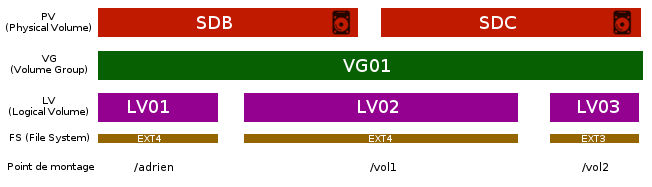
\includegraphics[width=15cm]{images/LVM.PNG}
        \caption{Représentation visuelle du LVM}
      \end{figure}
      \begin{itemize}[label = \textbullet, font = \Large]
        \item PV : Volumes physiques
        \begin{itemize}[label=\ding{228}, font=\scriptsize] 
          \item Les disques durs, partitions de disques durs, volumes RAID ou unités logiques provenant d'un SAN
        \end{itemize}
        \item VG : Groupes de Volumes
        \begin{itemize}[label=\ding{228}, font=\scriptsize] 
          \item Comme son nom l'indique, on crée un groupe comprenant plusieurs "PV" (Volumes physiques)
        \end{itemize}
        \item LV : Volumes logiques
        \begin{itemize}[label=\ding{228}, font=\scriptsize] 
          \item C'est comme une partition de VG
          \item On utilise le VG qui regroupe déjà plusieurs PV pour en faire le nombre de "partitions" (LV) que l'on souhaite. 
        \end{itemize}
        \item FS : File System
        \begin{itemize}[label=\ding{228}, font=\scriptsize] 
          \item Bien entendu, chaque LV doit comme pour une partition classique être formatée en un système de fichier pour être monté.
        \end{itemize}
      \end{itemize}

      \begin{itemize}[label = \textbullet, font = \Large]
        \item Le LVM (Logical Volume Manager) permet d'optimiser l'espace de nos différents disques (Voir Figure 2)
        \item Il apporte le stripping qui améliore les performances
        \item Les snapshots permettent de faciliter les sauvegardes
      \end{itemize}
      



      \section{Gestion Processus}
      Un processus a :
      \begin{itemize}[label = \textbullet, font = \Large]
        \item Un PID (Process ID, numéro du processus)
        \item Une priorité
        \item Un user propriétaire
        \item Un groupe propriétaire
      \end{itemize}
      Celui-ci a les même droits que son propriétaire (comme vu précédemment).

      \subsection{Afficher les processus}
      \begin{itemize}[label = \textbullet, font = \Large]
        \item \textsc{PS}
        \begin{itemize}[label=\ding{228}, font=\scriptsize] 
          \item Sans option, affiche les processus de l'utilisateur courant
          \item -u [user]
          \item -a all
          \item -x affiche les processus non rattaché à une console
          \item \textsc{ps aux} affiche donc tous les processus du système
        \end{itemize}
        \item Pstree
        \begin{itemize}[label=\ding{228}, font=\scriptsize] 
          \item Permet de visualiser la hiérarchie parent/enfant sous forme d'un "arbre" (ps\textbf{tree})
          \item Init est le 1er processus lancé
        \end{itemize}
        \item Top
        \begin{itemize}[label=\ding{228}, font=\scriptsize] 
          \item Permet de voir quel processus consomme le plus une certaine ressource
        \end{itemize}
        \item Pgrep
        \begin{itemize}[label=\ding{228}, font=\scriptsize] 
          \item Permet d'obtenir le PID (Process ID) d'un processus en mettant son nom comme argument
        \end{itemize}
      \end{itemize}

      \subsection{Interaction Processus}
      \begin{itemize}[label = \textbullet, font = \Large]
        \item Kill
        \begin{itemize}[label=\ding{228}, font=\scriptsize] 
          \item Envoie un signal à un ou plusieurs processus
          \item On peut utiliser le nom du processus ou son PID
          \item Les différents signaux :
          \begin{itemize}
            \item sighup (1) : relire les fichier de config
            \item sigint (2) : Interruption (Ctrl+C)
            \item sigquit (3) : Quit (Ctrl+D)
            \item sigkill (9) : Tue le processus immédiatement sans conditions
            \item sigterm (15) : Terminate (Demande de se terminer normalement)
            \item D'autres signaux dans la man page
          \end{itemize}
        \end{itemize} 
        \item Killall
        \begin{itemize}[label=\ding{228}, font=\scriptsize] 
          \item Permet d'envoyer un signal a un processus via son nom
          \item Par défaut, il s'agira du sigterm (15)
        \end{itemize}
        \item Pkill
        \begin{itemize}[label=\ding{228}, font=\scriptsize] 
          \item Comme Pgrep mais pour la gestion
        \end{itemize}
        \item Xkill
        \begin{itemize}[label=\ding{228}, font=\scriptsize] 
          \item Fait apparaître une tête de mort a la place de la souris
          \item Tue l'application dont la fenêtre est cliquée
        \end{itemize}
      \end{itemize}

      \subsection{Priorité}
      \begin{itemize}[label = \textbullet, font = \Large]
        \item Plus le chiffre est petit, plus il est important
        \item De -20 à 19
        \item 0 par défaut
        \item Seul root peut définir une priorité entre -20 et -1
        \item \textsc{nice -n []} permet de définir la priorité d'une application et de l'ouvrir
        \item \textsc{Renice} change la priorité d'un processus (Seul le propriétaire peut le faire)
      \end{itemize}

      \subsection{Contrôle des processus}
      \begin{itemize}[label = \textbullet, font = \Large]
        \item CTRL+C
        \begin{itemize}[label=\ding{228}, font=\scriptsize] 
          \item Arrêt
        \end{itemize}
        \item CTRL+z
        \begin{itemize}[label=\ding{228}, font=\scriptsize] 
          \item Pause
          \item Affiche la commande avec le numéro de job entre crochet
        \end{itemize}
        \item \textsc{fg}
        \begin{itemize}[label=\ding{228}, font=\scriptsize] 
          \item Permet de repasser en avant plan un processus
          \item Si on précise le numéro de job, c'est le processus correspondant au numéro qui repassera en avant plan
        \end{itemize}
        \item \textsc{bg}
        \begin{itemize}[label=\ding{228}, font=\scriptsize] 
          \item Laisse le "job" tourner en arrière-plan
        \end{itemize}
        \item \&
        \begin{itemize}[label=\ding{228}, font=\scriptsize] 
          \item Si placé lors de l'execution d'un job, celui-ci démarrera directement en arrière-plan
        \end{itemize}
        \item ;
        \begin{itemize}[label=\ding{228}, font=\scriptsize] 
          \item Permet de séparer plusieurs commandes les unes à la suite des autres
        \end{itemize}
        \item \&\&
        \begin{itemize}[label=\ding{228}, font=\scriptsize] 
          \item Executer une commande que si la précédente à réussi (a mettre entre les 2 commandes)
        \end{itemize}
      \end{itemize}

      \subsection{Planification}
      \begin{itemize}[label = \textbullet, font = \Large]
        \item cron
        \begin{itemize}[label=\ding{228}, font=\scriptsize] 
          \item composé de crond et crontab
          \item crond est le service qui va exécuter régulièrement les commandes voulues
          \item \textsc{/etc/crontab} est le fichier qui contient les commandes. (cron doit reboot si on modifie crontab)
          \item possibilité de placer des fichier crontab dans /etc/cron.d
          \item /etc/cron.hourly cron.daily cron.monthly contiennent les commandes que l’on veut exécuter toutes les heures, jours, mois
          \item cron ne lance pas les commandes dans un environnement complet. Faire attention a utiliser les chemins complets et initialiser ses propres variables si besoin
          \item Les scripts doivent commencer par un "\#"     
        \end{itemize}
        \item crontab
        \begin{itemize}[label=\ding{228}, font=\scriptsize] 
          \item Commande qui permet a chaque utilisateur d'éditer son fichier "crontab"
          \item Ouvre le crontab d'un utilisateur
          \item Configuration identique a \textsc{/etc/crontab}
          \item Cron vérifie le fichier toutes les minutes
          \item Les fichiers cron.allow et cron.deny permettent de gérer les autorisations (gère l'accès a crontab mais pas les tâches déjà planifiées)
          \item -e editer
          \item -l lister
          \item -r remove
          \item -u d'un utilisateur
        \end{itemize}
        \item Anacron
        \begin{itemize}[label=\ding{228}, font=\scriptsize] 
          \item Si le système est éteint à l’heure de l’exécution d’une tâche, elle ne sera pas exécutée. Anacron s’occupe de
          lancer ces actions
          \item Anacron est exécuté à intervalles réguliers par cron
        \end{itemize}
        \item At
        \begin{itemize}[label=\ding{228}, font=\scriptsize] 
          \item Passe au service atd des commandes à exécuter une seule fois à un moment précis
          \item Les accès peuvent être géré de la même manière que crontab
        \end{itemize}
      \end{itemize}

      \section{Etat du système (/proc)}
      \begin{itemize}[label = \textbullet, font = \Large]
        \item \textsc{/proc}
        \begin{itemize}[label=\ding{228}, font=\scriptsize] 
          \item Système de fichier virtuel (pas d'existence réelle)
          \item Créé et monté à chaque démarrage
          \item Permet de communiquer avec le kernel
          \item Donne la possibilté d'obtenir des informations mais aussi de modifier la configuration du noyau
          \item (Voir la synthèse du prof page 85-88 pour les différents fichiers de /proc)
        \end{itemize}
      \end{itemize}

      \section{Démarrage Linux}
      \begin{itemize}[label = \textbullet, font = \Large]
        \item Boot
        \begin{enumerate}[label=\ding{228}, font=\scriptsize] 
          \item Chercher, charger et executer le code de bootstrap (ex : BIOS)
          \item Pareil pour le kernel
          \item Executer les instructions de démarrage et les démons
          \item Gérer les processus et les états du stystème
        \end{enumerate}
        \item UEFI remplace BIOS
      \end{itemize}

      \subsection{UEFI - BIOS}
      \begin{enumerate}[label = \textbullet, font = \Large]
        \item Lors de la mise sous tension, le processeur est physiquement câblé de manière a charger et executer le code de démarrage situé a une adresse prédéterminé dans le NVRAM
        \item Pendant le bootstrapping, le firware va faire l'inventaire du matériel, l'initialiser et le vérifier
        \item Choisit un périphérique de démarrage (a partir de l'ordre de préférence pré-configuré)
        \item Démarre le système en chargeant le fichier de démarrage
      \end{enumerate}

      \subsubsection{UEFI}
      \begin{itemize}[label = \textbullet, font = \Large]
        \item Remplace le bios
        \item Peut se mettre en mode legacy pour être un supporté par un OS qui ne le supporte normalement pas
        \item Utilise des partitions GPT
        \item Peut interpréter le FS FAT
        \begin{enumerate}
          \item Le firmware cherche la partition "ESP" en FAT dans la GPT
          \item EFI est lu pour charger n'importe quel executable conçu pour être chargé pour l'UEFI (boot manager, GRUB, etc...)
        \end{enumerate}
        \item N'importe quel OS qui support le FAT peut editer l'ESP 
        \item Possibilité de consulter et de modifier UEFI sous linux grâce a l'API de UEFI (\textsc{efibootmgr})
      \end{itemize}

      \subsubsection{BIOS}
      \begin{itemize}[label = \textbullet, font = \Large]
        \item Firmware historique
        \item Souvent employé par défaut par les hyperviseurs
        \item Cherche les infos dans le BOOT LOADER (incapable de lire un FS)
      \end{itemize}

      \subsection{Boot Manager}
      \begin{itemize}[label = \textbullet, font = \Large]
        \item Anciennement appellé BootLoader
        \item Plus indispensables avec l'UEFI (capable de charger le kernel seul)
        \item Différents boot manager pour Linux
        \begin{itemize}[label=\ding{228}, font=\scriptsize] 
          \item GRUB 2 - Le plus répandu et celui utilisé par défaut
          \item Isolinux - démarrage sur CD, live usb, etc... 
          \item pxelinux - démarrage réseau
        \end{itemize}
      \end{itemize}

      \subsubsection{Configuration}
      \begin{itemize}[label = \textbullet, font = \Large]
        \item En général dans /boot/grub/
        \item Utiliser une partition séparée permet de d'utiliser un FS compréhensible pour GRUB et un autre FS pour le reste de l'arborescence
        \item Pour faciliter le multi-boot, la commande "os-prober" détecte les différents OS et les ajoute a GRUB
      \end{itemize}

      \subsection{Kernel Linux}
      \begin{itemize}[label = \textbullet, font = \Large]
        \item Initialisé avec les options passées en paramètres par le boot manager
        \item Réserve la mémoire et initialise les périphériques qu'il détecte
        \item Monte le FS racine et libère le ramdisk
        \item Lance le 1er processus : Systemd (gestion du système)
        \item Options passées au noyau
        \begin{itemize}[label=\ding{228}, font=\scriptsize] 
          \item debug
          \item racine : root=/dev/sda2
          \item mode single user : single
        \end{itemize}
        \item Possibilité de voir les messages du kernel quand il démarre grâce au logs et à \textsc{dmesg}
        \item Ne reste plus que lancer les processus qui tournent dans l'espace utilisateur
      \end{itemize}

      \subsection{Gestionnaire d'initialisation du système - Systemd}
      \begin{itemize}[label = \textbullet, font = \Large]
        \item Systemd remplace init et upstart
        \item Rôle : Faire tourner l'OS avec les bon daemons et paramètres de configuration
        \item Différents modes :
        \begin{itemize}[label=\ding{228}, font=\scriptsize] 
          \item single-user : sert pour le dépannage, fait le stricte minimum (et le seul utilisateur est root)
          \item multiuser : montages et services, multi-utilisateur et interface graphique
          \item server : comme multiuser mais en CLI
          \item reboot : redémarrage système
          \item etc...
        \end{itemize}
        \item Systemd est composé de nombreux executables, librairies et composants du kernel; ce qui le rend beaucoup plus intégré a l'OS que init qui n'est qu'un simple service.
        \begin{itemize}[label=\ding{228}, font=\scriptsize] 
          \item Comme dépendant au kernel Linux, il n'est pas portable sur d'autre "nixes" (comme MACOS)
          \item Peut ne pas supporter certaines version du kernel
        \end{itemize}
        \item Différences init / systemd
        \begin{itemize}[label=\ding{228}, font=\scriptsize] 
          \item runlevels remplacés par des "targets"
          \item Commande init sans intérêt
          \item inittab non existant
          \item Daemons géré par des fichiers de configuration ("units") et plus des scripts
          \item Systemd est conscient de ce qu'il se passe sur le système contrairement à init qui ne fait qu'executer des scripts
        \end{itemize}
        \item Units
        \begin{itemize}[label=\ding{228}, font=\scriptsize] 
          \item N'importe quel élément géré par systemd
          \item daemon, socket, timer, etc...
        \end{itemize}
        \item Systemctl
        \begin{itemize}[label=\ding{228}, font=\scriptsize] 
          \item Gestion de systemd (vérifier le status ou modifier sa configuration)
        \end{itemize}
      \end{itemize}

      \subsection{Init}
      \begin{itemize}[label = \textbullet, font = \Large]
        \item Encore utilisé sur les distributions devant être légères
        \item 1er processus lancé : /sbin/init (lance le système grâce au fichier de configuration /etc/inittab)
        \item rcS est un script lancé par init qui va lancer les différents scripts dans "rcS.d" qui vont gérer les éléments de base du système (initialisation clavier, hostname, monter les partitions etc...)
        \item Fini par initialiser le runlevel par défaut puis démarre les consoles
      \end{itemize}

      \subsubsection{RunLevels}
      \begin{itemize}[label = \textbullet, font = \Large]
        \item Peut varier selon la distribution
        \item Par convention :
        \begin{itemize}[label=\ding{228}, font=\scriptsize] 
          \item 1 : mode single user
          \item 0 : éteindre le système
          \item 6 : redémarrage systèmes
        \end{itemize}
        \item Sous Debian :
        \begin{itemize}[label=\ding{228}, font=\scriptsize] 
          \item 2 : multiuser (par défaut)
          \item 3-4-5 : Non utilisé
        \end{itemize}
        \item RedHat :
        \begin{itemize}[label=\ding{228}, font=\scriptsize] 
          \item 2 : multiuser sans NFS
          \item 3 : multiuser
          \item 4 : non utilisé
          \item 5 : multiuser + GUI (par défaut)
        \end{itemize}
        \item Pour changer le runlevel par défaut : "init" et "telinit" ou lors du démarrage (grâce au Boot Manager)
      \end{itemize}

      \subsubsection{/etc/init.d}
      \begin{itemize}[label = \textbullet, font = \Large]
        \item Contient tous les scripts de démarrage de service
        \item Pour s'adapter au runlevel, différents liens symboliques sont crées dans les répertoires rc0.d $\rightarrow$ rc6.d
        \begin{itemize}[label=\ding{228}, font=\scriptsize] 
          \item Commencent par un "S" si service à démarrer 
          \item Commencent par un "K" si service à arrêter
          \item Suivi du numéro d'ordre de démarrage
          \item ex : S20networking
        \end{itemize}
        \item Les fichiers de configuration des scripts de démarrage de init.d sont dans /etc/default (/etc/sysconfig sur redHat)
      \end{itemize}

      \subsubsection{Problème d'init}
      \begin{itemize}[label = \textbullet, font = \Large]
        \item Scripts RC pas tous compatibles avec certaines modules
        \item execute des scripts sans se préoccuper du système
        \item Nombreux scripts sur chaque runlevel
        \item Difficile de lancer un service suite à une action ou de relander automatiquement un service
        \item Travail dupliqué d'une distribution à l'autre (doit y être intégré)
        \item Difficilement modifiable par l'utilisateur
        \item Pas de gestion de dépendances
        \item Pas de parallèlisme (pas compris ce point)
      \end{itemize}

      \section{Gestion du kernel}
      \subsection{Rôle du kernel}
      \begin{itemize}[label = \textbullet, font = \Large]
        \item gérer les processus
        \item gérer les périphériques
        \item gérer les INPUT/OUTPUT
        \item gérer les interruptions
        \item gérer les ressources
        \item gérer les FS
      \end{itemize}

      \subsection{Type de kernel}
      \begin{itemize}[label = \textbullet, font = \Large]
        \item monolithique
        \begin{itemize}[label=\ding{228}, font=\scriptsize] 
          \item Le kernel forme un gros bloc de code qui gère tous les rôles
        \end{itemize}
        \item microkernel
        \begin{itemize}[label=\ding{228}, font=\scriptsize] 
          \item Le noyau est minimal et le maximum des features sont déportés sous dorme de serives dans l'espace utilisateur
        \end{itemize}
        \item hybride
        \begin{itemize}[label=\ding{228}, font=\scriptsize] 
          \item microkernel dont toutes les features ne sont pas externalisé (gain de perfs)
        \end{itemize}
        \item Linux est monolithique modulaire (les modules peuvent être chargé/déchargé)
      \end{itemize}

      \subsection{Version du noyau}
      \begin{itemize}[label = \textbullet, font = \Large]
        \item Commande \textsc{uname}
        \begin{itemize}[label=\ding{228}, font=\scriptsize] 
          \item Forme : (NuméroMajeur).(NuméroMineur).(NiveauDePatch)
          \item Numéro mineur :
          \begin{itemize}
            \item Impair $\rightarrow$ version de développement
            \item Pair $\rightarrow$ version stable
          \end{itemize}
        \end{itemize}
      \end{itemize}

      \subsection{Modules}
      Morceau de code pouvant être chargé/déchargé du noyau
      \begin{itemize}[label = \textbullet, font = \Large]
        \item /lib/modules/version\char`_kernel/ (extension .ko)
        \item Risque perte de performance et de sécurité
        \item \textsc{lsmod} liste les modules actifs
        \item \textsc{modinfo} info sur un module
        \item \textsc{insmod} charger un module
        \item \textsc{modprobe} charger un module en gérant ses dépendances
        \item \textsc{rmmod} désinstaller un module
        \item Possibilité de spécifier les modules à charger lors du démarrage grâce au boot manager
      \end{itemize}

      \subsection{Compilation}
      \begin{itemize}[label = \textbullet, font = \Large]
        \item gcc
        \begin{itemize}[label=\ding{228}, font=\scriptsize] 
          \item Compilateur C
        \end{itemize}
        \item make
        \begin{itemize}[label=\ding{228}, font=\scriptsize] 
          \item outils pour gérer la compilation
        \end{itemize}
      \end{itemize}


      \section{PAM}
      \textbf{Merci a Thibaut Watrisse pour ses notes}\\
      \textbf{P}luggable \textbf{A}uthentification \textbf{M}odules
      \begin{itemize}[label = \textbullet, font = \Large]
        \item Ensemble des librairies qui servent à fournir une authentification flexible sur un systèmme UNIX
        \item Réponse au soucis des développeur devant mettre en place un mécanisme d'authentification pour leur application
        \item L’administrateur va pouvoir changer comme il l’entend de mécanisme d’authentification, du moment que le module PAM nécessaire existe
        \item But de PAM : Séparer le dev. des applications de celui du mécanisme d'authentification sécurisé
      \end{itemize}

      \subsection{Fonctionnement de PAM}
      \begin{itemize}[label = \textbullet, font = \Large]
        \item Login
        \begin{itemize}[label=\ding{228}, font=\scriptsize] 
          \item vérifie que l'utilisateur est bien celui qu'il prétend être
          \begin{itemize}
            \item Login appelle PAM, puis PAM va lire ses fichiers de config et charge ensuit les modules appropriés
          \end{itemize}
          \item  L’échange de messages avec l’utilisateur (envoyés ou reçus) est effectué à travers l’application via la fonction conversation()
          \item fournit le shell tournant avec l'identité de l'utilisateur
        \end{itemize}
        \item Gère l'authentification, les comptes, les sessions, les mdp
      \end{itemize}

      \begin{figure}[H]
        \centering
        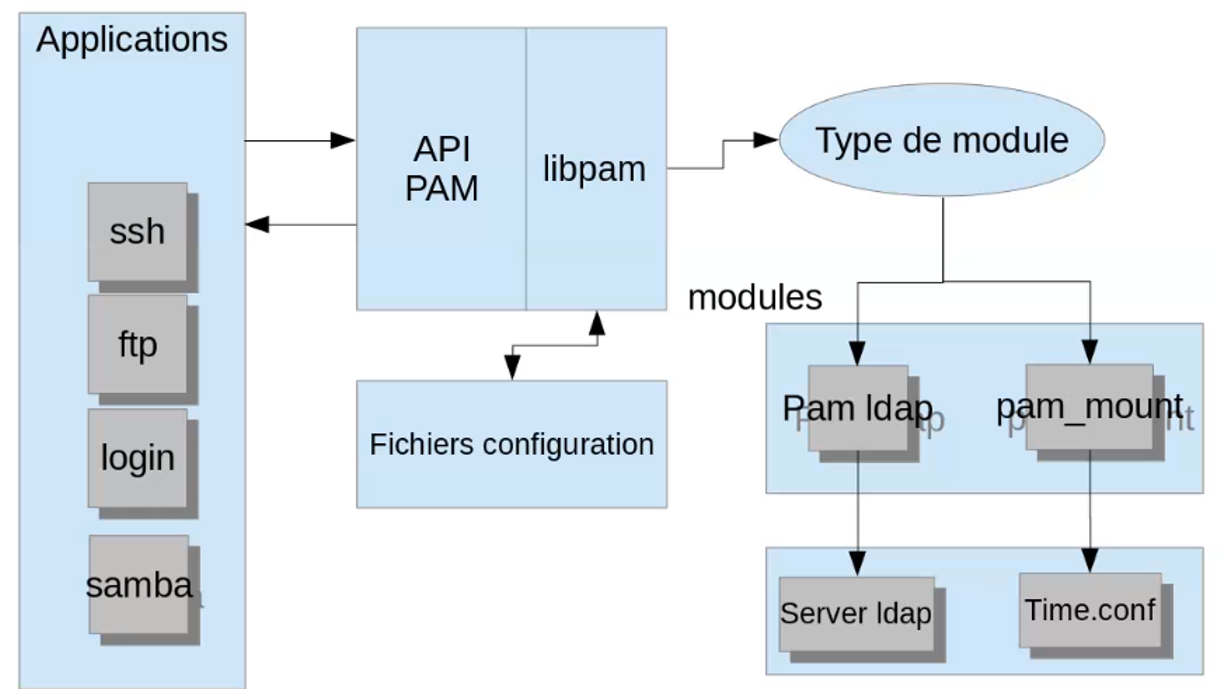
\includegraphics[width=15cm]{images/PAM.PNG}
        \caption{Représentation visuelle du LVM}
      \end{figure}

      \subsection{Config.}
      \begin{itemize}[label = \textbullet, font = \Large]
        \item Librairies
        \begin{itemize}[label=\ding{228}, font=\scriptsize] 
          \item /lib/security
          \item /lib64/security
        \end{itemize}
        \item Fichiers de config.
        \begin{itemize}[label=\ding{228}, font=\scriptsize] 
          \item /etc/pam.d
          \item /etc/pam.conf
        \end{itemize}
        \item Fichiers de config. des modules
        \begin{itemize}[label=\ding{228}, font=\scriptsize] 
          \item /etc/security
        \end{itemize}
        \item Chaque application utilisant PAM correspond un fichier dans pam.d portant le nom du service concerné
        \item Structure fichier pam
        \begin{itemize}[label=\ding{228}, font=\scriptsize] 
          \item [service] type\char`_module contrôle\char`_chemin\char`_module arguments\char`_module
        \end{itemize}
        \item Conseil :
        \begin{itemize}[label=\ding{228}, font=\scriptsize] 
          \item Si erreur dans la configuration $\rightarrow$ échec de PAM
          \item Prendre ses précautions lors de modifications dans un fichier de configuration
        \end{itemize}
        \item Différents types de modules
        \begin{itemize}[label=\ding{228}, font=\scriptsize] 
          \item auth
          \begin{itemize}
            \item sert à authentifier l'utilisateur
            \item donne l'appartenance aux groupes (ou autres privilèges)
          \end{itemize}
          \item account
          \begin{itemize}
            \item Tâche d'un compte (sauf authentification)
            \item ex : restreindre l'accès a certaines heures, les ressources, etc...
          \end{itemize}
          \item session
          \begin{itemize}
            \item environnement
            \item monter des répertoires
            \item création d'un répertoire personnel
            \item (Tout ce qui est lié a une session)
          \end{itemize}
          \item password
          \begin{itemize}
            \item ce module est requis pour mettre à jour les données d’authentification de l’utilisateur
            \item Possibilité de mettre en place des stratégies de mdp
          \end{itemize}
        \end{itemize}
        \item Flags :
        \begin{itemize}[label=\ding{228}, font=\scriptsize] 
          \item requisite
          \begin{itemize}
            \item En cas d’échec, l’information est retournée directement, et les modules suivants ne sont pas parcourus
          \end{itemize}
          \item sufficient
          \begin{itemize}
            \item Si réussite, envoie directement le message de réussite à l’application sans tester les modules suivants
            \item Si échec, pas d’importance, sauf s’il s’agit du dernier module de la pile.
          \end{itemize}
          \item optionnal
          \begin{itemize}
            \item  PAM passera au
            module suivant dans la pile que ce soit un échec ou une réussite
          \end{itemize}
        \end{itemize}
      \end{itemize}

      \subsection{Modules}
      \begin{center}
        \begin{tabular}{|l|r|}
          \hline
          \makecell[c]{\textbf{Module}} & \makecell[c]{\textbf{Description}}\\
          \hline
          pam\char`_console &  \makecell[l]{Permet de donner à des user des droits qu’ils n’auraient pas autrement }\\
          \hline
          pam\char`_access & \makecell[l]{Limite l’accèes sur base de critères supplémentaires que le critère d’authentification}\\
          \hline
          pam\char`_cracklib & \makecell[l]{Vérification des mdp (imposer une taille, caractères spéciaux,…)}\\
          \hline
          pam\char`_deny & \makecell[l]{Sert à retourner un échec}\\
          \hline
          pam\char`_ftp & \makecell[l]{Permet l’accès anonyme sur FTP}\\
          \hline
          pam\char`_issue & \makecell[l]{Pour afficher un petit message avant de demander le login}\\ 
          \hline
          pam\char`_limits & \makecell[l]{Donne des limites dans les ressources utilisateur}\\ 
          \hline
          pam\char`_listfile & \makecell[l]{Permet d’autoriser(ou pas) sur base d’un fichier}\\ 
          \hline
          pam\char`_mount & \makecell[l]{Permet de monter un système de fichier distant}\\ 
          \hline
          pam\char`_mkhomedir & \makecell[l]{Permet de créer un répertoire personnel}\\ 
          \hline
          pam\char`_nologin & \makecell[l]{Vérifie qu’un fichier nologin existe dans etc ou pas, si c’est le cas, il n’y a que root qui peut se connecter}\\ 
          \hline
          pam\char`_permit & \makecell[l]{Renvoie automatiquement « succes » }\\ 
          \hline
          pam\char`_rootok & \makecell[l]{Permet à root d’avoir accès à certains services sans taper le mdp}\\ 
          \hline
        \end{tabular}\\
      \end{center}

      \section{Radius}
      \textbf{Merci a Thibaut Watrisse pour l'aide des notes}\\
      \textbf{R}emote \textbf{A}uthentification \textbf{D}ial-\textbf{I}n \textbf{U}ser \textbf{S}service (Dial-in = composer)\\[0.2cm]
      Exemple de mise en place d'une authentification radius qui m'a aidé à mieux comprendre :\\ https://www.youtube.com/watch?v=abIOD4O4AJg\\[0.2cm]

      \begin{itemize}[label = \textbullet, font = \Large]
        \item UDP Port 1812
        \item But de radius
        \begin{itemize}[label=\ding{228}, font=\scriptsize]
          \item Va permettre l'authentification à un service de manière individualisé
          \item Exemple : Au lieu d'utiliser une seule clé WiFi, chaque employé à son propre accès au service WiFi
        \end{itemize}
        \item Serveur
        \begin{itemize}[label=\ding{228}, font=\scriptsize]
          \item Gère l'authentification
          \item Utilise une base de donnée d'Identification (.txt, SQL, LDAP, etc..)
          \begin{itemize}
            \item Peut être propre au serveur Radius ou bien la base de donnée d'un Active Directory par exemple
          \end{itemize}
        \end{itemize}
        \item Client
        \begin{itemize}[label=\ding{228}, font=\scriptsize]
          \item NAS (Network Acces Server)
          \item Pour n'importe quel service demandant une authentification
          \item Par exemple : Un routeur Wifi
        \end{itemize}
        \item Fonctionnement
        \begin{itemize}[label=\ding{228}, font=\scriptsize]
          \item Le client radius va s'authentifier auprès du serveur Radius avec une clé PSK (clée partagée)
          \begin{itemize}
            \item La sécurité entre le serveur et le client est assurée par cette clée qui crypte notamment le mot de passe de l'utilisateur
          \end{itemize}
          \item L'utilisateur contacte le client Radius pour une demande d'authentification
          \item Le client radius traite la demande d'authentification auprès du serveur Radius
        \end{itemize}
        \item Protocoles
        \begin{itemize}
          \item EAP
          \begin{itemize}[label=\ding{228}, font=\scriptsize]
            \item Extensible Authentication Protocol
            \item 802.1x = intégration de EAP dans la couche 2
          \end{itemize}
        \end{itemize}
        \item MDP
        \begin{itemize}[label=\ding{228}, font=\scriptsize]
          \item PAP
          \begin{itemize}
            \item Simple authentification par mot de passe
            \item Password Authentication Protocol
            \item Le user envoie son login et mdp en clair
            \item Le serveur renvoie soit un \textsc{authentication-ack} si OK, sinon un \textsc{authentication-nack}
          \end{itemize}
          \item CHAP
          \begin{itemize}
            \item Challenge-Handshake Authentication Protocol
            \item 4 types de paquets : Challenge, Reponse, Succès, Echec
            \begin{enumerate}
              \item L'authentificateur envoie un challenge au client (Access-Challenge)
              \item Celui-ci répond avec une valeur calculée à l'aide d'une fonction de hashage (Access-Request)
              \item L'authentificateur vérifie la réponse par rapport à son propre calcul
              \item Si les hash correspondent, alors l'authentificateur reconnaît l'authentification
              \item Le challenge est renouvelé à des intervales random par sécurité
            \end{enumerate}
          \end{itemize}
        \end{itemize}
        \item Extensions Microsoft
        \begin{itemize}[label=\ding{228}, font=\scriptsize]
          \item Mschap
          \item Mschapv2
        \end{itemize}
        \item Problèmes : Sécurité des échanges faible
        \begin{itemize}[label=\ding{228}, font=\scriptsize]
          \item Solution :
          \begin{itemize}
            \item Protéger les flux de données via VPN
            \item Privilégier des méthodes sûre entre user et client
          \end{itemize}
        \end{itemize}
      \end{itemize}

      \section{Kerberos}
      \textbf{Merci a Thibaut Watrisse pour l'aide des notes}\\
      Rôle : Fournir un système d'authentification unifié en milieu hétérogène (pour n'importe quel client, serveur,...)

      \begin{itemize}[label = \textbullet, font = \Large]
        \item Authentication
        \begin{itemize}[label=\ding{228}, font=\scriptsize]
          \item De manière sûre
          \item De manière centralisée (Single Sign On - SSO)
        \end{itemize}
        \item CAS
        \begin{itemize}[label=\ding{228}, font=\scriptsize]
          \item Central Authentication Service
          \item Mdp centralisé dans un AD (ou autre système)
          \item Permet de se connecter sur divers services avec nos mêmes identifiants
        \end{itemize}
        \item SSO - Single Sign On
        \begin{itemize}[label=\ding{228}, font=\scriptsize]
          \item Plus avancé que "CAS"
          \item Lors de la connexion, on reçoit un jeton pendant un certain temps nous permettant de nous connecter a nos différents services sans passer par la case "authentification"
        \end{itemize}
      \end{itemize}

      \subsection{Protocole Needham et Schroeder}

      \begin{itemize}[label = \textbullet, font = \Large]
        \item A = Alice
        \item B = Bob
        \item S = Tiers parti de confiance
        \item K = Key
        \item $K_{BS}$ = Key partagée entre Bob et le tiers parti de confiance
        \item $N_x$ = Nombre aléatoire généré par $x$
      \end{itemize}

      \begin{figure}[H]
        \centering
        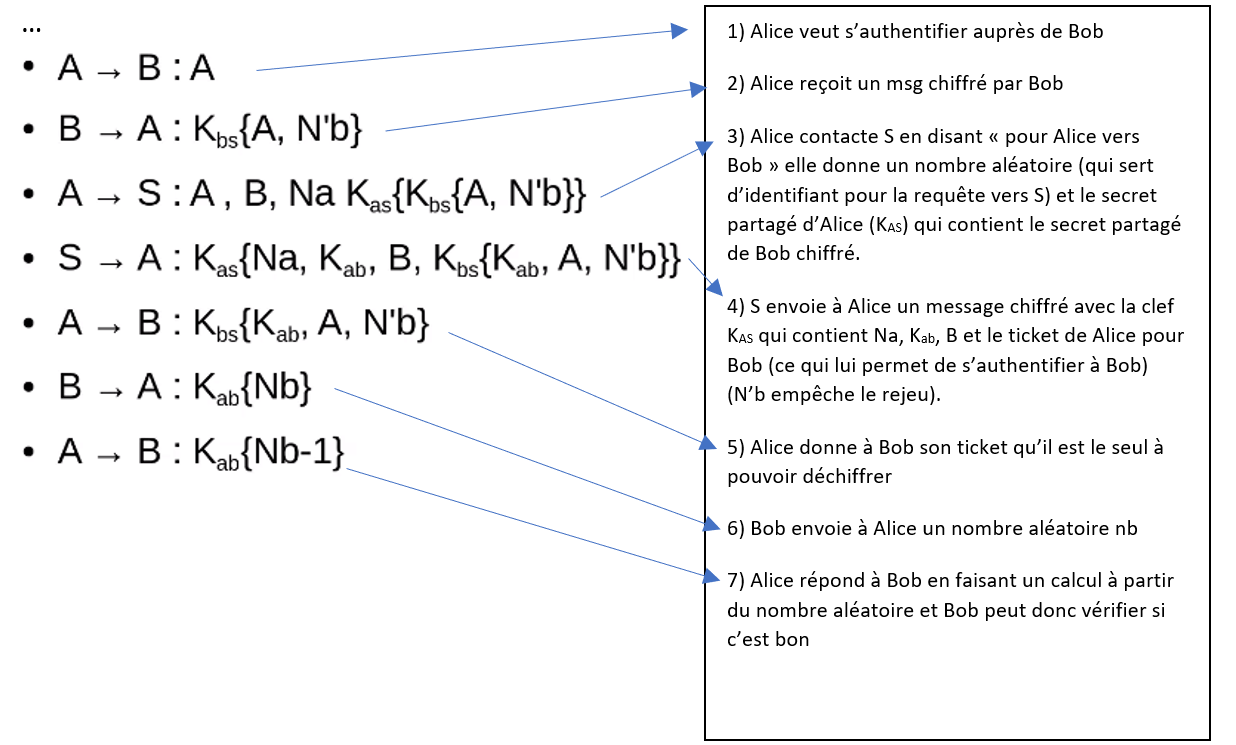
\includegraphics[width=15cm]{images/aie.PNG}
        \caption{Etapes (Image de Watrisse Thibaut)}
      \end{figure}

      Etant donné qu'il est difficile de générer des vrais nombres aléatoires avec Kerberos, on utilise donc des "Time Stamp"

      \begin{itemize}[label = \textbullet, font = \Large]
        \item KDC
        \begin{itemize}[label=\ding{228}, font=\scriptsize]
          \item Le tiers parti de confiance
          \item Génère un "royaume" kerberos (kerberos realm)
          \item Divisé en 2 services
          \begin{itemize}
            \item TGS - Ticket Granting Server qui fourni les tickets
            \item AS - Authentication Service auprès duquel les clients s'authentifient
          \end{itemize}
        \end{itemize}
        \item Une fois connecté à l'AS, on peut demander des tickets au TGS
        \begin{itemize}[label=\ding{228}, font=\scriptsize]
          \item Les clefs secrètes sont les hash des mdp $K_a$
          \item Anti-rejeu
          \begin{itemize}
            \item Time Stamp
            \item Durée de vie des tickets
          \end{itemize}
        \end{itemize}
        \item Etant donné qu'on utilise des time stamp, toutes les machines doivent être configuré à la même geure
        \item Différence d'heure max sur un active diretory : max 5 min.
      \end{itemize}

      \subsection{En résumé}

      \begin{itemize}
        \item REQ = Request
        \item REP = Reply
        \item AS = Authentication Service
        \item TGS = Ticket Granting Server
        \item Bob = Service
        \item Alice = Utilisateur
      \end{itemize}

      \begin{figure}[H]
        \centering
        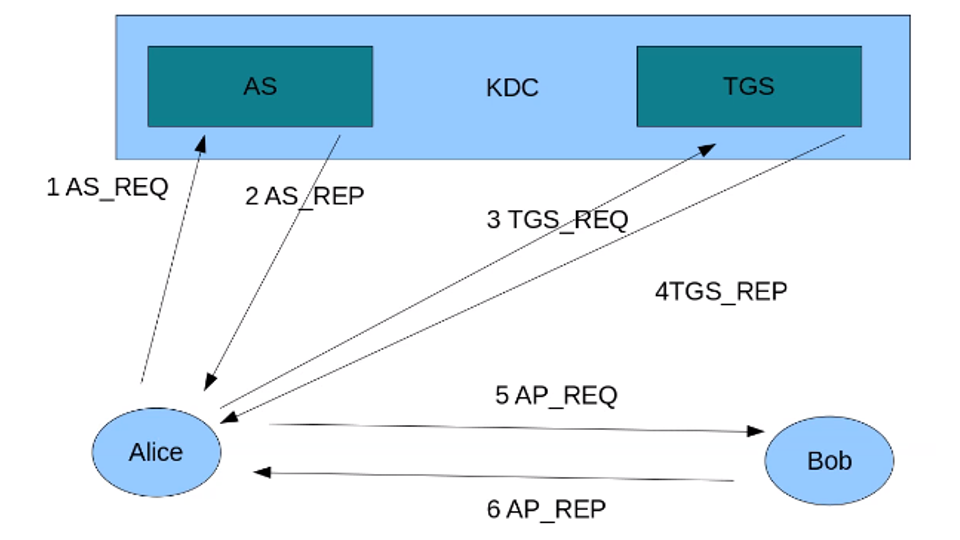
\includegraphics[width=12cm]{images/TGS.PNG}
        \caption{Fonctionnement de Kerberos}
      \end{figure}

      \begin{enumerate}
        \item Alice s'authentifie dans le royaume Kerberos (Demande d'un TGT)
        \begin{itemize}[label=\ding{228}, font=\scriptsize]
          \item A $\rightarrow$ AS : A, ticketlifetime,[$K_a$\{timestamp\}]
          \item Pré authentification optionnelle
          \begin{itemize}
            \item Si il n’y a pas de pré authentification l’AS n’est pas sûr que c’est elle mais ce n’est pas important car si ce n’est pas Alice, 
            elle ne comprendra pas la réponse de l’AS car l’usurpateur ne connaitra pas le secret partagé.
          \end{itemize}
        \end{itemize}
        \item AS envoie la durée de vie du ticket et la session key (TGT - Ticket Granting Ticket) entre ALice et le TGS
        \begin{itemize}[label=\ding{228}, font=\scriptsize]
          \item AS $\rightarrow$ A : $K_a$\{Ticket lifetime, $K_{a,tgs}$\}
          \item AS $\rightarrow$ A : $K_{tgs}$\{A, timestamp, $K_{a,tgs}$,ticket lifetime\}
        \end{itemize}
        \item Alice contacte TGS (Demande d'un TS)
        \begin{itemize}[label=\ding{228}, font=\scriptsize]
          \item A $\rightarrow$ TGS : $K_{a,tgs}$\{A, timestamp, ticket lifetime\}
          \begin{itemize}
            \item Le TGS saura grâce au TGT que ça vient d'Alice
          \end{itemize}
        \end{itemize}
        \item TGS répond à la demande pour le service bob avec un ticket de service TS
        \begin{itemize}[label=\ding{228}, font=\scriptsize]
          \item TGS $\rightarrow$ A : $K_{a,tgs}$\{Bob, timestamp, ticket lifetime\}
          \item TGS $\rightarrow$ A : $K_{b}$\{Alice, Bob, $K_{ab}$, timestamp, ticket lifetime\}
        \end{itemize}
        \item Alice s'authentifie auprès de Bob
        \begin{itemize}
          \item A $\rightarrow$ B : $K_{ab}$\{A, timestamp, ticket lifetime\}
          \item B $\rightarrow$ A : $K_{ab}$\{timestamp - 1\}
          \begin{itemize}
            \item La réponse de Bob va permettre de vérifier que le timestamp n'a pas déjà été utilisé (rejeu)
            \item Bob peut alors déchiffrer le message d'Alice grâce à TS qui contient la clef de session entre Alice et Bob
            \item Une fois le message déchiffré, Bob est sensé voir apparaître l'ID d'Alice, le Ticket Lifetime, et le timestamp
          \end{itemize}
        \end{itemize}
      \end{enumerate}

      \subsection{Points Negatifs}

      \begin{itemize}
        \item Dépendances au temps
        \item Si KDC tombe en panne, plus possible de s'authentifier nulle part (Single point of failure)
        \item Si mdp compromis, alors KDC est compris aussi (Solution : Passer par des certificats)
        \item Les services doivent supporter Kerberos
        \item Il faut utiliser des algorithme symétrique fort (AES par exemple)
      \end{itemize}
      \newpage
      \tableofcontents





























\end{document}